\documentclass{article}

% if you need to pass options to natbib, use, e.g.:
%     \PassOptionsToPackage{numbers, compress}{natbib}
% before loading neurips_2020

% ready for submission
% \usepackage{neurips_2020}

% to compile a preprint version, e.g., for submission to arXiv, add add the
% [preprint] option:
%     \usepackage[preprint]{neurips_2020}

% to compile a camera-ready version, add the [final] option, e.g.:
%     \usepackage[final]{neurips_2020}

%     to avoid loading the natbib package, add option nonatbib:
\PassOptionsToPackage{numbers, sort, compress}{natbib}
\usepackage{neurips_2020}

\usepackage[utf8]{inputenc} % allow utf-8 input
\usepackage[T1]{fontenc}    % use 8-bit T1 fonts
\usepackage{hyperref}       % hyperlinks
\hypersetup{draft} % weird pdfendlink error
\usepackage{url}            % simple URL typesetting
\usepackage{booktabs}       % professional-quality tables
\usepackage{amsfonts}       % blackboard math symbols
\usepackage{nicefrac}       % compact symbols for 1/2, etc.
\usepackage{microtype}      % microtypography
\usepackage{amsmath, amsfonts, amssymb, amsthm}

\usepackage{color}
\definecolor{darkblue}{rgb}{0.0,0.0,0.2}
\hypersetup{colorlinks,breaklinks,
	linkcolor=darkblue,urlcolor=darkblue,
	anchorcolor=darkblue,citecolor=darkblue}
\usepackage{wrapfig}
\usepackage{subcaption}
\usepackage[colorinlistoftodos,textsize=tiny]{todonotes} % need xargs for below
%\usepackage{accents}
\usepackage{bbm}
\usepackage{xspace}

\newcommand{\Comments}{1}
\newcommand{\mynote}[2]{\ifnum\Comments=1\textcolor{#1}{#2}\fi}
\newcommand{\mytodo}[2]{\ifnum\Comments=1%
	\todo[linecolor=#1!80!black,backgroundcolor=#1,bordercolor=#1!80!black]{#2}\fi}
\newcommand{\raf}[1]{\mynote{green!80!blue}{[RF: #1]}}
\newcommand{\raft}[1]{\mytodo{green!20!white}{RF: #1}}
\newcommand{\jessie}[1]{\mynote{purple}{[JF: #1]}}
\newcommand{\jessiet}[1]{\mytodo{purple!20!white}{JF: #1}}
\newcommand{\proposedadd}[1]{\mynote{orange}{#1}}
\newcommand{\bo}[1]{\mynote{blue}{[Bo: #1]}}
\newcommand{\botodo}[1]{\mytodo{blue!20!white}{Bo: #1}}
\newcommand{\btw}[1]{\mytodo{gray!10!white}{\textcolor{gray}{BTW: #1}}}%TURN OFF FOR NOW \mytodo{gray}{#1}}
\ifnum\Comments=1               % fix margins for todonotes
\setlength{\marginparwidth}{1in}
\fi

\newcommand{\reals}{\mathbb{R}}
\newcommand{\posreals}{\reals_{>0}}%{\reals_{++}}
\newcommand{\simplex}{\Delta_\Y}
\newcommand{\relint}[1]{\mathrm{relint}(#1)}
\newcommand{\prop}[1]{\mathrm{prop}[#1]}
\newcommand{\elic}{\mathrm{elic}}
\newcommand{\eliccvx}{\mathrm{elic}_\mathrm{cvx}}
\newcommand{\elicpoly}{\mathrm{elic}_\mathrm{pcvx}}
\newcommand{\elicembed}{\mathrm{elic}_\mathrm{embed}}
\newcommand{\ccdim}{\mathrm{cc\,dim}}
\newcommand{\codim}{\mathrm{codim}}
\newcommand{\rank}{\mathrm{rank}}
\newcommand{\supp}{\mathrm{supp}}
\newcommand{\spn}{\mathrm{span}}
\newcommand{\propdis}{\mu}
\newcommand{\affhull}{\mathrm{affhull}}
\newcommand{\epi}{\mathrm{epi}}


\newcommand{\C}{\mathcal{C}}
\newcommand{\D}{\mathcal{D}}
\newcommand{\E}{\mathbb{E}}
\newcommand{\F}{\mathcal{F}}
\renewcommand{\L}{\mathfrak{L}}
\newcommand{\I}{\mathcal{I}}
\newcommand{\N}{\mathcal{N}}
\newcommand{\R}{\mathcal{R}}
\renewcommand{\P}{\mathcal{P}}
\newcommand{\Sc}{\mathcal{S}}  % jessie, feel free to redef, just not \S :-)
\newcommand{\U}{\mathcal{U}}
\newcommand{\X}{\mathcal{X}}
\newcommand{\Y}{\mathcal{Y}}


\newcommand{\ellbar}{\underline{\ell}}
\newcommand{\lbar}{\underline{L}} % couldn't do L* while proofreading...
\newcommand{\iden}{\mathrm{iden}}
\newcommand{\Var}{\mathrm{Var}}

\newcommand{\exploss}[3]{\E_{#3} #1(#2,Y)}
\newcommand{\risk}[1]{\underline{#1}}
\newcommand{\inprod}[2]{\langle #1, #2 \rangle}
\newcommand{\toto}{\rightrightarrows}
\newcommand{\ones}{\mathbbm{1}}

\newtheorem{theorem}{Theorem}
\newtheorem{lemma}{Lemma}
\newtheorem{proposition}{Proposition}
\newtheorem{corollary}{Corollary}
\newtheorem{conjecture}{Conjecture}
\newtheorem{definition}{Definition}
\newtheorem{assumption}{Assumption}
\newtheorem{remark}{Remark}


\DeclareMathOperator*{\argmax}{arg\,max}
\DeclareMathOperator*{\argmin}{arg\,min}
\DeclareMathOperator*{\arginf}{arg\,inf}
\DeclareMathOperator*{\sgn}{sgn}

\usepackage{thmtools, thm-restate}
%\declaretheorem{corollary}


\title{Indirect elicitation as a necessary condition for consistent surrogate losses}

% The \author macro works with any number of authors. There are two commands
% used to separate the names and addresses of multiple authors: \And and \AND.
%
% Using \And between authors leaves it to LaTeX to determine where to break the
% lines. Using \AND forces a line break at that point. So, if LaTeX puts 3 of 4
% authors names on the first line, and the last on the second line, try using
% \AND instead of \And before the third author name.

\author{%
  Jessie Finocchiaro\\
%  Department of Computer Science\\
  CU Boulder\\
  \texttt{jefi8453@colorado.edu} 
  % examples of more authors
  \And
   Rafael Frongillo\\
%   Department of Computer Science\\
   CU Boulder\\
  % Address \\
   \texttt{raf@colorado.edu} 
   \And
   Bo Waggoner\\
%   Department of Computer Science\\
   CU Boulder \\
  % Address \\
   \texttt{bwag@colorado.edu} 
  % \And
  % Coauthor \\
  % Affiliation \\
  % Address \\
  % \texttt{email} \\
  % \And
  % Coauthor \\
  % Affiliation \\
  % Address \\
  % \texttt{email} \\
}



\begin{document}

\maketitle

\begin{abstract}
Given a prediction task, understanding when one can and cannot design a consistent convex surrogate loss, particularly a low-dimensional one, is an important and active area of machine learning research. 
While calibration has historically been used to reason about consistency, we propose indirect property elicitation as an alternative necessary condition for a surrogate loss to be consistent. 
Motivated by structured prediction and other domains where the prediction dimension of the surrogate is of central importance, we give a novel lower bound on the prediction dimension. 
Our lower bound tightens existing results in the case of discrete predictions, namely the feasible subspace dimension, showing that previous work implicitly relied on calibration only via property elicitation. 
For continuous predictions, our lower bound gives new results for variance estimation as well as the estimation of entropy and norms of the conditional distribution.
\end{abstract}

\section{Introduction}\label{sec:intro}

Surrogate risk minimization is one of the most widespread techniques in supervised machine learning.
A surrogate loss is often necessary for one of two reasons: (1) the target loss does not satisfy some desiderata, such as convexity, or (2) the target loss may not be given at all, as is often the case in continuous estimation problems, when one instead has a target conditional statistic to estimate from training data.
In both of these settings, a minimal requirement of a surrogate loss is \emph{consistency}, a precursor to excess risk bounds and rates.
Roughly speaking, consistency means that minimizing surrogate risk corresponds to solving the target problem of interest:
the target risk should also be minimized, or the average deviation to and true conditional statistic function converges to 0.

Motivated by structural prediction and other problems with exponentially or infinitely large label sets, we are particularly interested in the \emph{prediction dimension} of a surrogate: the dimension $d$ of its prediction space $\reals^d$.
A natural tension arises between consistency and the prediction dimension, as consistency is always possible for a sufficiently large dimension, but a larger dimension typically increases the computational complexity of learning.
We are therefore interested in finding consistent convex surrogates with a low prediction dimension, such as logarithmic in the number of labels, as is desired in many structured prediction problems~\cite{ramaswamy2018consistent,yu2018lovasz,berman2018lovasz}.
%\raft{FYI Jessie: what used to be this last paragraph still didn't quite get where you want to be in terms of motivating the problem.  I'd suggest taking a careful look at the diff at some point to see what I changed and ask me if you don't see why.  Probably the biggest issue was in laying out the gap.  You often need to give more detail about what \emph{has} been done to say what hasn't.}

While meaningful bounds on the prediction dimension have recently begun to appear, both for discrete and continuous predictions~\cite{lambert2008eliciting,ramaswamy2016convex,ramaswamy2018consistent,frongillo2018elicitation}, these works have several drawbacks.
Consistency for discrete target losses is typically studied using calibration, which though powerful and undeniably useful, can be challenging to work with, and general results about calibration are sparse.
In the case of continuous predictions, results for \emph{convex} surrogates remain a major open problem~\cite{frongillo2018elicitation}.

Our results make two contributions toward closing this gap.
First, after introducing a general definition of consistency (\S~\ref{sec:consis-implies-indir}) which applies to all four settings mentioned above, we show that indirect property elicitation is a necessary condition for consistency in all these settings (Theorem~\ref{thm:consistent-implies-indir-elic}).
As indirect elicitation is more tractable than calibration, and applies more generally, this observation suggests indirect elicitation as the better choice to study lower bounds on the prediction dimension of a consistent surrogate.
Second, we state a general lower bound on the prediction dimension of a consistent \emph{convex} surrogate (Theorem~\ref{thm:cvx-flats}).
Our result generalizes a calibration result of \citet{ramaswamy2016convex} to all four settings, yielding to our knowledge the most general such bound.

While indirect elicitation is only a necessary condition, our bounds recover or improve upon the state of the art:
we achieve tighter bounds than the feasible subspace dimension approach for discrete predictions~\citep{ramaswamy2016convex}, yet recover their result (Corollary~\ref{cor:fsd-bound}), and no bounds for convex surrogates were known in the continuous prediction setting~\citep{frongillo2018elicitation}.
Furthermore, in all of the examples we consider, our lower bounds match the best upper bounds.
For these reasons, we advocate for indirect elicitation as a tractable and more general alternative to calibration when studying the consistency of surrogates.

%We typically use convex surrogate loss functions that take some input $u \in \reals^d$ and measure error against the observed outcome $y \in \Y$.
%The value $d$ provides some notion of efficiency for the surrogate, as low-dimensional convex losses can improve the efficiency of the optimization algorithm.
%\cite{frongillo2015elicitation} pose an open question regarding a general characterization of the efficiency of \emph{convex elicitable properties}, which we show is bounded by finding the minimum dimension $d$ for which a consistent, convex loss can be constructed for the task at hand.

% After reviewing previous work and tools to study consistency (\S~\ref{sec:related-work}), we lay down a new general definition of consistency which can simultaneously capture all four settings mentioned above (\S~\ref{sec:consis-implies-indir}).
% Our main result (\S~\ref{sec:char-convex}, Theorem~\ref{thm:cvx-flats}) provides a necessary condition for
% the existence of consistent convex surrogates in a given dimension $d$.
% This result is closely related to those provided by~\citet[Theorem 16]{ramaswamy2016convex} in the discrete prediction setting; in fact, we show their result is a special case of our main result (Corollary~\ref{cor:fsd-bound}).
% We illustrate our main result with several examples (\S~\raf{examples}), one of which addresses an open question posed by~\citet[Section 8]{frongillo2018elicitation} in the continuous estimation setting.
%\raft{FYI: use citet when treating citations as nouns; citep is used when the citation does not participate in the grammar, like: ``That is funny [Noah Alexander Frongillo, personal communication, 5/31/2020].''  Not sure what 'cite' does in this style...}\jessiet{Noted, and propogated}


\section{Background and Related work}\label{sec:related-work}

We consider supervised learning problems in the space $\X \times \Y$, for some \emph{feature space} $\X$ and a finite \emph{label space} $\Y$, with data drawn from a distribution $D$ over $\X \times \Y$.
The task is to produce a hypothesis $f: \X \to \R$, for some \emph{prediction space} $\R$, which may be different from $\Y$.
For example, in ranking problems $\R$ may be all $n!$ permutations over the $n$ labels forming $\Y$.
As we focus heavily on conditional distributions $D_x = \Pr[Y|X=x]$ over $\Y$ given some $x \in X$, we often abstract away $x$, working directly with probability simplex $\simplex$, the set of all distributions over $\Y$.

If given, we use $\ell: \R \times \Y \to \reals$ to denote a \emph{target loss}, with predictions $r\in\R$.
%where the goal is minimize expected loss, $\E ~ \ell(f(X),Y)$ for pairs $X,Y$ drawn from some distribution.
Similarly, $L: \reals^d \times \Y \to \reals$ will typically denote a \emph{surrogate} loss, with surrogate predictions $u \in \reals^d$.
A loss $\ell$ is \emph{discrete} if $\R$ is a finite set.
A surrogate $L$ is \emph{convex} if $L(\cdot,y)$ is convex for every label $y \in \Y$.
For a given $p\in\simplex$, the (conditional) \emph{regret}, or excess risk, of a loss $L$ is given by $R_L(u,p) := \exploss{L}{u}{p} - \inf_{u^*} \exploss{L}{u^*}{p}$.

\botodo{Define calligraphic L, L sub d for dimension d.}

\btw{Add note about minnability}
% For a distribution $p \in \simplex$, we denote the expected target loss for prediction $r$ to be $\E_{Y \sim p} \ell(r, Y) := \ell(r; p)$.
% Similarly, $\E_{Y \sim p} L(u, Y) := L(u ; p)$.



\subsection{Consistency} \label{subsec:consistency}


%\bo{Citation help appreciated!} \jessie{\cite{fisher1922mathematical,zhang2004statistical,bartlett2006convexity,tewari2007consistency,steinwart2007compare,ramaswamy2016convex} -- these are the ones I know of that discuss consistency in slightly various forms.  I believe the definition we run with is most similar to \cite{ramaswamy2016convex}.}
A basic requirement of surrogate losses $L: \reals^d \times \Y \to \reals$ is consistency, which roughly means that minimizing $L$-loss corresponds to solving the target problem of interest.
We consider two kinds of consistency.
In the first, we are given a \emph{target loss} $\ell$, and we roughly define $L$ to be consistent if minimizing $L$, and applying a link, minimizes $\ell$ (Definition \ref{def:consistent-ell}).
This definition follows much of the machine learning literature~\citep{zhang2004statistical,bartlett2006convexity,tewari2007consistency,steinwart2007compare,ramaswamy2016convex}.
In the second, we are given a \emph{target statistic}, such as the conditional variance or quantile, as in classical statistics~\citep{fisher1922mathematical}.
Here we will define $L$ to be consistent if minimizing $L$ and applying a link function yields estimates converging to the correct value, by some measure (Definition \ref{def:consistent-prop}).

In addition to the two possible targets, we may have one of two domains: a \emph{discrete} (i.e.\ finite) target prediction space, like a classification problem, or a \emph{continuous} one, like a regression or estimation problem.
We informally refer to the four resulting cases---target loss vs.\ statistic, and discrete vs.\ continuous predictions---as the ``four quadrants'' of supervised learning problems.

The goal of this paper is to give lower bounds on the dimension $d$ of consistent surrogate losses.
A priori, it is not necessarily clear that compatible definitions of consistency could be given for both target statistics and target losses.
We observe that, in fact, target losses are a special case of target statistics (\S~\ref{sec:consis-implies-indir}),
which suggests property elicitation (see \S~\ref{subsec:properties}) as being uniquely suited to studying general lower bounds.
% This technique will then allow us to prove lower bounds across all four quadrants.
In prior work, most research on this problem focuses on the quadrant of target losses and discrete predictions~\citep{zhang2004statistical,bartlett2006convexity,tewari2007consistency,ramaswamy2015hierarchical,ramaswamy2016convex,ramaswamy2018consistent}.
%\raft{Jessie: add cites here?}\jessie{done}
In particular, as definitions of consistency are relatively intractable to apply directly, the literature often focuses on a weaker condition called calibration, which only applies when given a discrete target loss.


\subsection{Calibration}\label{subsec:calibration}

When given a discrete target loss, such as for classification-like problems, direct empirical risk minimization is typically NP-hard, forcing one to find a more tractable surrogate.
To ensure consistency, the literature has embraced the notion of \emph{calibration} due to~\citet{tewari2007consistency}, and its generalizations to arbitrary discrete target losses~\citep{agarwal2015consistent,ramaswamy2016convex}.
Calibration is a much more tractable and weaker condition than consistency, yet the two are equivalent under suitable assumptions~\cite{tewari2007consistency,ramaswamy2016convex}.
Intuitively, calibration says that one cannot approach the optimal surrogate loss while linking to an suboptimal target prediction.
%\raft{FYI Jessie: what you had was now pretty redundant to what we have earlier}\jessie{Definitely}

% For discrete prediction problems, we often start with a target loss $\ell$ in mind: for classification, 0-1 loss comes to mind; for high-confidence classification, a variation of 0-1 loss that allows a constant, moderate penalty for abstaining can be used.
% However, optimizing over a target loss is often a computationally hard problem.
% This is why we use surrogate losses, but desire consistency to guarantee the surrogate ``corresponds'' to the original loss.%, or property we want to predict, as is more common in the the continuous estimation setting.
% A surrogate is no good on its own; we also need a link function to map from the surrogate prediction space back to the \emph{correct} prediction in the original prediction space.
% This notion of a correct surrogate is typically captured by the notion of \emph{consistency}, introduced formally in Definitions~\ref{def:consistent-ell} and~\ref{def:consistent-prop}.
% Related, and sometimes equivalent, is \emph{calibration}, which was the primary tool to study consistency until~\citet{agarwal2015consistent} introduced the use of property elicitation to study consistency in certain contexts.

\begin{definition}[Calibrated: discrete predictions]\label{def:calibrated-finite}
	Let $\ell : \R \times \Y \to \reals$ be a discrete target loss, and let $\gamma : \simplex \to 2^\R$ be given by $\gamma(p) = \argmin_{r\in\R} \exploss{\ell}{r}{p}$.
	A surrogate loss $L : \U \times \Y \to \reals$  and link $\psi:\U \to \R$ pair $(L, \psi)$ is \emph{calibrated with respect to} $\ell$ if 
	\begin{equation}\label{eq:calibration}
	\forall p \in \simplex: \inf_{u \in \U : \psi(u) \not \in \gamma(p)} \exploss{L}{u}{p} > \inf_{u \in \U} \exploss{L}{u}{p}~.~
	\end{equation}
\end{definition}
Typically, we take $\U = \reals^d$ for some $d\in\mathbb{N}$.
\btw{We could also replace $\U$ by $\reals^d$ throughout, but it seemed distracting in this section}

Many works characterize calibrated surrogates for specific discrete target losses~\citep{zhang2004statistical,lin2004note,bartlett2006convexity,tewari2007consistency}, including the canonical 0-1 loss for binary and multiclass classification.
Moreover, \citet{steinwart2007compare} and \citet{steinwart2008support} generalize the study of consistent losses from the discrete prediction setting and characterizes different types of loss functions, relating excess risk bounds, consistency, and calibration for various classes of surrogate losses (i.e. margin-based, distance-based, supervised, unsupervised, etc.).
%See~\citet[Chapter 2]{steinwart2008support} for further discussion of these loss functions.
In Appendix~\ref{app:calibration}, we give a definition of calibration which is equivalent to Definition~\ref{def:calibrated-finite} in discrete prediction settings, but generalizes to continuous estimation settings.\jessiet{Suggest trimming down if needed}


\subsection{Property elicitation}\label{subsec:properties}
\btw{Don't be too braggy}
Arising from the statistics and economics literature, property elicitation is similar to calibration, but only places a restriction on the exact minimizers of a surrogate~\citep{savage1971elicitation,osband1985information-eliciting,lambert2008eliciting,lambert2009eliciting,lambert2018elicitation,frongillo2015vector-valued,frongillo2014general}.
Specifically, given a statistic or \emph{property} $\Gamma$ of interest, which maps a distribution $p$ over $\Y$ to the set of desired or correct predictions, the minimizers of $L$ should precisely coincide with $\Gamma$.
Intuitively, $p = \Pr[Y|X=x]$ is a conditional distribution, though the definition is also applied to point prediction settings.
%\raft{FYI Jessie: I like this line but $D_x$ has not been defined yet \jessie{I added $D$ in the notation section and introduced it there.  Let me know if it really doesn't mesh with you, but I think it fit somewhat naturally.}}

\begin{definition}[Property, elicits]
	A \emph{property} is a set-valued function $\Gamma : \simplex \to 2^\R \setminus \{\emptyset\}$, which we denote $\Gamma: \simplex \toto \R$.
	A loss $L : \R \times \Y \to \reals$ \emph{elicits} the property $\Gamma$ if
	\begin{equation}
    \label{eq:elic}    
    \forall p \in \simplex, \;\; \Gamma(p) = \argmin_{u \in \R} \exploss{L}{u}{p}~.
	\end{equation}
\end{definition}

The \emph{level set} of $\Gamma$ at value $r\in\R$ is $\Gamma_r := \{p \in \simplex : r \in \Gamma(p)\}$.
We call a property $\Gamma: \simplex \toto \R$ \emph{discrete} if $\R$ is a finite set.
A property is \emph{single-valued} if $|\Gamma(p)| = 1$ for all $p\in\simplex$, in which case we write $\Gamma\to\R$.
We use $\Gamma := \prop{L}$ to denote the unique property elicited by $L$ from eq.~\eqref{eq:elic}.
Finally, when multiple properties are in play, we typically denote the target property by $\gamma$, and the surrogate by $\Gamma$.

To relate property elicitation to consistency, we need to allow for a link function, which gives rise to the notion of \emph{indirect} elicitation.
\begin{definition}[Indirect Elicitation]\label{def:indirectly-elicits}
	A loss and link $(L, \psi)$ \emph{indirectly elicit} a property $\gamma:\simplex \toto \R'$ if $L$ elicits a property $\Gamma: \simplex \toto \U$ such that for all $u \in \U$, we have $\Gamma_u \subseteq \gamma_{\psi(u)}$.
	We say $L$ \emph{indirectly elicits} $\gamma$ if such a link $\psi$ exists.
\end{definition}
For single-valued properties, the above definition reduces to the natural requirement $\gamma = \psi \circ \Gamma$.
\btw{interesting discussion of set-valued properties commented out; revive later!}
% While there are several possible set-valued extensions, Definition~\ref{def:indirectly-elicits} best matches  suited for studying consistency.
% There are a few possible definitions of indirect elicitation, but this is the most applicable for our setting because when we consider set-valued properties, we do not have that \emph{all} optimal predictions for $\Gamma$ must be linked back to \emph{all} optimal predictions for $\gamma$.
% Instead, we lighten this restriction to say that any optimal prediction for $\Gamma$ must be linked to \emph{an} optimal prediction for $\gamma$, and we must do so deterministically. 

It is straightforward to show that, for a discrete target loss $\ell$, calibration implies indirect elicitation, as perhaps first observed by \citet{agarwal2015consistent}.
Formally, if $(L,\psi)$ is calibrated with respect to $\ell$, then $(L,\psi)$ indirectly elicits $\gamma = \prop{\ell}$.
To see this, take $u\in\U$ and $p\in\Gamma_u$, implying $u\in\Gamma(p)$.
From eq.~\eqref{eq:elic}, $\exploss{L}{u}{p} = \inf_{u'\in\U} \exploss{L}{u'}{p}$, so we must have $\psi(u) \in \gamma(p)$ from eq.~\eqref{eq:calibration}, as desired.
%\raft{Jessie: if this argument makes sense to you, you can cut that prop in the appendix now}
As a result, indirect elicitation in a necessary condition for consistency when given a target discrete loss.
As we will see in \S~\ref{sec:consis-implies-indir}, it is also a necessary condition for consistency more broadly, including in all four quadrants mentioned above.

An important caveat to the above definitions is that we have required $\Gamma = \prop{L}$ to be nonempty everywhere, meaning that $\exploss{L}{\cdot}{p}$ always achieves a minimum.
\raft{Let's make sure we agree with this paragraph}
While this condition technically rules out several popular surrogates such as logistic and exponential loss for binary classification, these can be included for example by thresholding the loss $L'(u,y) = \max(L(u,y),\epsilon)$ for sufficiently small $\epsilon>0$.
\botodo{work on ``heavily impacted''}
The results in this paper are not heavily impacted by this restriction, as for example assuming $\Gamma(p) \neq \emptyset$ whenever $p\in\relint\simplex$ is strong enough to include the above examples without impacting Theorems~\ref{thm:cvx-flats} and~\ref{thm:bayes-risk-lower-bound}.
\raft{In particular, I'm torn about whether this statement is accurate; in the sense that we can restrict to $\P\subseteq\simplex$ I think it's fair, but in the sense that calibration does not imply indirect elicitation without it, perhaps not.}
We expect that a generalization of property elicitation which allows for ``infinite'' predictions (e.g., along a prescribed ray), thereby ensuring a minimum is always achieved for convex losses, would allow us to lift this restriction entirely.
\btw{Some refs / related work commented out here.  I think not as relevant as elicitation complexity.}

% Property elicitation of a single property is well-understood~\citep{savage1971elicitation,osband1985information-eliciting,lambert2008eliciting, lambert2009eliciting, lambert2018elicitation}, and \citet{finocchiaro2018convex} are among the first to consider \emph{convex} elicitable properties.
% Additionally, \citet{agarwal2015consistent} are the first to our knowledge to formally relate property elicitation to the consistency of a surrogate loss, although they only consider settings with $|\Y| < \infty$. \jessiet{right?}
%However, their assumptions are more restrictive than ours; they only consider losses defined on the real line.% and assume the properties to be identifiable: an assumption we do not need.


\subsection{Prediction dimension and elicitation complexity}\label{subsec:complexity}

Various works have studied the minimum prediction dimension $d$ needed in order to construct a consistent surrogate loss $L: \reals^d \times \Y \to \reals$, typically through proxies such as calibration~\citep{agarwal2015consistent,ramaswamy2016convex} and property elicitation~\citep{frongillo2015vector-valued,fissler2016higher,frongillo2018elicitation}.
%\raft{Nice!  Love ``proxies'' here.}
In the case of a discrete target loss, \citet{ramaswamy2016convex} introduce \emph{convex calibration dimension}, the minimum prediction dimension yielding a convex calibrated surrogate.
Their results has led to the design of consistent convex surrogates for discrete prediction problems such as hierarchical classification~\citep{ramaswamy2015hierarchical} and classification with an abstain option~\citep{ramaswamy2018consistent}.
%\raft{FYI Jessie: Two general points.  (1) I spent the majority of my time in this section just on dependencies; e.g.\ you had ``similar to elicitation complexity mentioned above'' but elicitation complexity was not mentioned above.  Next time it would be more efficient if you made sure to balance local edits with global scans to catch these sorts of things, as well as making sure we aren't explaining things twice, etc.  (2) You tend to mix background with nods to our results, which is actually good to do, but it can be jarring if you go back and forth too much.  See for example how I changed the previous subsection, reserving the nod to our work to the end of the subsection.}\jessiet{Noted boss man}

\btw{Take out of definition environment?}
\begin{definition}[Convex Calibration Dimension]
	Given a target discrete loss $\ell$, its \emph{convex calibration dimension} $\ccdim(\ell)$ is the minimum dimension $d$ such that there is a convex surrogate \mbox{$L: \reals^d \times \Y \to \reals$} and link $\psi$ such that $(L,\psi)$ is calibrated with respect to $\ell$.
\end{definition}
\btw{Now we'll introduce a different notion, which is related to calibration.}

In the case of a target statistic/property $\gamma$, \citet{lambert2008eliciting} similarly introduce the notion of \emph{elicitation complexity}, later generalized by \citet{frongillo2018elicitation}, which captures the lowest prediction dimension of a surrogate which indirectly elicits $\gamma$.
This notion is more general as it extends to continuous estimation settings and does not inherently depend on a target loss being given. 
% However, until now, no formal connection to consistency has been shown for convex elicitation complexity.

\begin{definition}[Convex Elicitation Complexity]
	Given a target property $\gamma$, the \emph{convex elicitation complexity} $\eliccvx(\gamma)$ is the minimum dimension $d$ such that there is a convex surrogate \mbox{$L : \reals^d \times \Y \to \reals$} indirectly eliciting $\gamma$.
\end{definition}

\btw{cut this? but still want to answer the question of ``how does elicitation relate to calibration?''}
As we show next, calibration implies indirect elicitation, which means the convex elicitation complexity always lower bounds the convex calibration dimension in the setting of discrete target losses.
Yet despite this fact, the state-of-the-art lower bound for convex calibration dimension, the \emph{feasible subspace dimension} of \citet{ramaswamy2016convex}, is a special case of our lower bound for convex elicitation complexity (Theorem~\ref{thm:cvx-flats}), meaning we achieve the same or even higher lower bounds.
(See the examples in \S~\ref{subsec:examples-finite}.)
Moreover, convex elicitation complexity also applies beyond the discrete target loss setting, as we demonstrate in \S~\ref{sec:contin-consis}.

In related work,
\citet{finocchiaro2019embedding} study surrogate losses which \emph{embed} a discrete loss in some sense, which is a special case of indirect elicitation.
They construct a calibrated link functions from embeddings, which together with observations about indirect elicitation, imply that for polyhedral (piecewise linear and convex) losses, calibration and indirect elicitation are equivalent.
\citet{finocchiaro2020embedding} further introduce the notion of \emph{embedding dimension}, which is a lower bound on both convex elicitation complexity of discrete properties and convex calibration dimension of discrete losses.
Since embedding is a special case of indirect elicitation, we have the chain of inequalities, embedding dimension $\leq$  ``polyhedral calibration dimension'' $\leq$ convex calibration dimension; it is an open problem whether any of these inequalities can be strict.


\section{Consistency implies indirect elicitation}\label{sec:consis-implies-indir}

In this section, we show that indirect elicitation is necessary for consistency (Theorem \ref{thm:consistent-implies-indir-elic}) for losses in $\L$, while simultaneously applying to all of the above settings (our four quadrants).
For the case of a given discrete target loss, it is well-known that a surrogate is consistent if and only if it is calibrated (e.g.\,~\citep[Theorem 1, part 3]{bartlett2006convexity}).
For this case, we can show Theorem~\ref{thm:consistent-implies-indir-elic} via calibration, and even extend the definition of calibration and proof approach to continuous prediction spaces.
As we are also interested in the other two quadrants, when given a target statistic instead of as target loss,
we delegate this proof to Appendix~\ref{app:calibration} and directly prove the general result for all four quadrants.

Since indirect elicitation is implied by both consistency and calibration of a surrogate $L \in \L$, it might seem a very weak necessary condition for consistency.
Yet, as we show in the following sections, it gives state-of-the-art lower bounds on the prediction dimension of consistent convex surrogates.
In particular, we will derive bounds that imply those given by the feasible subspace dimension approach (Corollary~\ref{cor:fsd-bound}).


We start by formalizing consistency in two ways that generalize across our four quadrants.
First, given an target loss $\ell$, then we say $L$ is consistent if optimizing $L$ implies optimizing $\ell$ (Definition~\ref{def:consistent-ell}).
Second, given a target property $\gamma$, such as the $\alpha$-quantile, we say $L$ is consistent if optimizing $L$ implies approaching, in some sense, the correct statistic $\gamma(D_x)$ of the conditional distributions $D_x = \Pr[Y|X=x]$ (Definition~\ref{def:consistent-prop}).
We then observe that Definition~\ref{def:consistent-ell} is subsumed by Definition~\ref{def:consistent-prop}, and use this to show consistency always implies $L$ indirectly elicits $\prop{\ell}$ or $\gamma$ respectively.

\begin{definition}[Consistent: loss]\label{def:consistent-ell}
	A loss and link $(L,\psi)$ are consistent with respect to an target loss $\ell$ if, for all distributions $D$ over input and label spaces $\X \times\Y$, and for all sequences of measurable hypothesis functions $\{f_m : \X \to \R\}$,
	\begin{align*}
	\E_D L(f_m(X), Y) \to \inf_f \E_D L(f(X), Y) &\implies \E_D \ell((\psi \circ f_m)(X), Y) \to \inf_f \E_D \ell((\psi \circ f)(X), Y)~.~
	\end{align*}
\end{definition}
%% Bo: resolved, Jun 1
%\botodo{On the right side, is measurable enough? I guess we need $\psi \circ f$ to be measurable...on the other hand, we don't want to constrain $f$ based on $\psi$. Do we need a condition on $\psi$ that guarantees $\psi \circ f$ is measurable?}
%\raft{I think okay as written -- if $\psi$ is restrictive, you won't achieve consistency.  And typically $f$ is much more expressive anyway, e.g. $\reals^\Y$ for classification.}

Instead of a target loss $\ell$, one may want to learn a conditional statistic such as the expected value, variance, or entropy.
In this case, following the tradition in the statistics literature on conditional estimation~\citep{gyorfi2006distribution,fan1998efficient,ruppert1997local},
we formalize consistency as converging to the correct conditional estimates of the property.
Convergence is measured by functions $\propdis(r, p)$ that formalize how close $r$ is to ``correct'' for conditional distribution $p$.
In particular we should have $\propdis(r,p) = 0 \iff r \in \gamma(p)$.
\btw{Bo: Would be nice to give some natural special cases: for a finite property, $\propdis(r,p) = \mathbf{1}[r \in \gamma(p)]$, and for single-valued properties with a distance metric on $\R$, $\propdis(r,p) = \text{dist}(r, \gamma(p))$.}

\begin{definition}[Consistent: property]\label{def:consistent-prop}
	Suppose we are given a loss $L : \R \times \Y \to \reals$, link function $\psi: \R \to \R'$, and property $\gamma:\simplex \toto \R'$.
	Moreover, let $\propdis : \R' \times \simplex \to \reals_+$ be any function satisfying $\propdis(r,p) = 0 \iff r \in \gamma(p)$.
	We say $(L, \psi)$ is \emph{$\mu$-consistent with respect to} $\gamma$ if, for all distributions $D$ over $\X \times \Y$, and for all sequences of measurable functions $\{f_m: \X \to \R\}$, 
	\begin{equation}
    \E_{D} L(f_m(X), Y) \to \inf_f \E_{D} L( f(X), Y) \implies \E_X \propdis(\psi \circ f_m(X), D_X) \to 0~,
  \end{equation}
  where $D_x = \Pr[Y|X=x]$.
	We say $(L,\psi)$ is consistent with respect to $\gamma$ if there is such a $\propdis$ so that $(L,\psi)$ is $\propdis$-consistent with respect to $\gamma$.
\end{definition}

%Theorem~\ref{thm:consistent-implies-indir-elic} shows that consistency, either with respect to a target loss $\ell$ or a property $\gamma$, implies indirect elicitation.

If $\gamma$ is a property elicited by a target loss $\ell$, then taking $\propdis$ to be the regret with respect to $\ell$, the two definitions are equivalent. % for the appropriate choice of $\propdis$.
% when using target regret of $r$ (compared to an optimal prediction for $p$) as $\propdis(r,p)$.
\begin{lemma}\label{lem:consistent-loss-implies-prop}
	Given a surrogate loss $L$, link $\psi$, and target loss $\ell$, set
	% Take $\propdis: \R \times \simplex \to \reals_+$ with 
  $\mu(r,p) := R_\ell(r,p)$.
  Then
	$(L, \psi)$ is consistent with respect to $\ell$ if and only if $(L,\psi)$ is $\propdis$-consistent with respect to $\gamma := \prop{\ell}$.
  \btw{Note: don't actually $\gamma$ nonempty here.}
\end{lemma}
\begin{proof}
	First, observe that $\propdis(r,p) = 0 \iff \exploss{\ell}{r}{p} = \inf_{r' \in \R} \exploss{\ell}{r'}{p} \iff r \in \gamma(p)$.
	Now suppose $(L, \psi)$ are consistent with respect to $\ell$, and take any sequence $\{f_m\}$ of measurable hypotheses.
  Rewriting the right-hand side of Definition~\ref{def:consistent-ell},
        \begin{align}
	  &\; \E_D \ell(\psi \circ f_m(X), Y)\to \inf_f \E_D \ell(\psi \circ f(X), Y)   \label{eqn:cons-loss-cond} \\
	  &\iff \E_X R_\ell(\psi \circ f_m(X), D_X) \to 0                               \nonumber  \\
	  &\iff \E_X \propdis(\psi \circ f_m(X), D_X) \to 0~.~                          \label{eqn:cons-prop-cond}
	\end{align}
        Therefore, $\mathbb{E}_D L(f_m(X),Y) \to \inf_f \mathbb{E}_D L(f(X),Y)$ implies (\ref{eqn:cons-loss-cond}) if and only if it implies (\ref{eqn:cons-prop-cond}).
\end{proof}

When noting that some properties are not elicitable, including the variance, Lemma~\ref{lem:consistent-loss-implies-prop} confirms that consistency with respect to a property is a strictly broader notion, and further points to indirect elicitation as a natural necessary condition for consistency.
We now show this necessity directly.

\begin{theorem}\label{thm:consistent-implies-indir-elic}
	For a surrogate $L \in \L$, if the pair $(L, \psi)$ is consistent with respect to a property $\gamma$ or loss $\ell$ eliciting $\gamma$, then $(L, \psi)$ indirectly elicits $\gamma$.
\end{theorem}
\begin{proof}
%  \raft{Maybe ref the consistency definition here explicitly, at the top and the end}
	By Lemma~\ref{lem:consistent-loss-implies-prop}, it suffices to show the result for consistency with respect to a property $\gamma$, setting $\gamma := \prop{\ell}$ if $\ell$ is given instead.
	We show the contrapositive; suppose $(L, \psi)$ does not indirectly elicit $\gamma$, meaning we have some $p \in \simplex$ so that $u \in \Gamma(p)$ but $\psi(u) \not \in \gamma(p)$, where $\Gamma := \prop{L}$.
	Observe that we use the fact $\Gamma(p) \neq \emptyset$.
	Consider the constant sequence $\{f_m\}$ with $f_m(x) = u$ for all $m,x$, and take $D$ with full support on some $x \in \X$, and let $D_x = p$.
  Since $u \in \Gamma(p)$, we observe $\E_D L(f_m(X), Y) = \inf_f L(f(X),Y)$ for all $m$; in particular $\E_D L(f_m(X), Y) \to \inf_f L(f(X),Y)$.
%  \raft{Maybe clearer to first say $\E_D L(f_m(X), Y) = \inf_f L(f(X),Y)$ for all $m$, and then the easy implication of the convergence \jessie{Done}}
	However, we have $\E_X \propdis(\psi \circ f_m(X), D_X) = \propdis(\psi(u_m), p) = \propdis(\psi(u), p) \neq 0$, since $\psi(u) \not \in \gamma(p)$.
%  \raft{Almost -- just clarify that this is the expectation over $D$ too by construction \jessie{Kinda done?}}
	Thus, we observe $(L, \psi)$ is not consistent with respect to $\gamma$ (Definition~\ref{def:consistent-prop}).
\end{proof}

\section{Prediction Dimension of Consistent Convex Surrogates}\label{sec:char-convex}

We now turn to the question of bounding the prediction dimension of a consistent convex surrogate.
From Theorem \ref{thm:consistent-implies-indir-elic}, given a target property $\gamma$ or loss $\ell$ with $\gamma = \prop{\ell}$, this task reduces to lower bounding the prediction dimension of a convex surrogate indirectly eliciting $\gamma$.
We now explore a tool, Theorem \ref{thm:cvx-flats}, for proving such convex-elicitation lower bounds.
The key idea, crystallized from the proof of \citet[Theorem 16]{ramaswamy2016convex}, is to consider a particular distribution~$p$ and surrogate prediction $u \in \reals^d$ with is optimal for $p$.
Theorem \ref{thm:cvx-flats} will show that if $d$ is small, then the level set $\{p : u \in \argmin_{u'} \exploss{L}{u'}{p}\}$ must be large; in fact, it must roughly contain a high-dimensional affine subspace, or \emph{flat}.
But by definition of indirect elicitation, there is some level set $\gamma_r$ (where $u$ is linked to $r$) containing this flat as well.
The point of this result is the contrapositive: if $\gamma$ has a level set intricate enough to not contain any high-dimensional flats, then $\gamma$ cannot have a low-dimensional consistent surrogate.

We now define flats formally.
Recall that the affine hull is the set of all linear combinations whose coefficients sum to 1.
In particular, we will often use $\affhull(\simplex) = \{\sum_{i=1}^n \alpha_i p_i : p_i \in \simplex, \alpha_i \in \reals, \sum_{i=1}^n \alpha_i = 1\}$, which has dimension $n-1$.
\begin{definition}[Flat]\label{def:flat}
	A \emph{flat} $F \subseteq \affhull(\simplex) \subseteq \reals^n$ is a nonempty set $F = \ker W \cap \affhull(\simplex)$ for some $W\in\reals^{d\times n}$ where $d\leq n$.
	The codimension of $F$ (relative to $\affhull(\simplex)$) is given by $\codim(F)=\mathrm{rank}(W)$, and the dimension of $F$ is $n - \mathrm{rank}(W) - 1$.
\end{definition}


We now state our lower bound.

\begin{theorem}\label{thm:cvx-flats}
  Let a property $\gamma:\simplex\toto\R$ be given, let $p\in\simplex$ such that either (i) $|\gamma(p)|=1$ or (ii) $\gamma$ is elicitable and $p\in\relint\simplex$, and let $r\in\gamma(p)$.
Then if $L: \reals^d \times \Y \to \reals$ indirectly elicits $\gamma$, there is a flat $F$ with $p\in F \cap \simplex \subseteq \gamma_r$ and $\codim(F) \leq d$.
% COmmented 06.03.20
%	If there is a convex surrogate loss $L : \reals^d \times\Y \to \reals$ indirectly eliciting $\gamma$, then for all $p \in \simplex$ and $r \in \R$ such that $r \in \gamma(p)$, there is a flat $F \subseteq \affhull(\simplex)$ of codimension at most $d$ such that $F \cap \simplex \subseteq \gamma_r$ and $p \in F$.
\end{theorem}
\begin{proof}

%	There is some u in Gamma(p). (Gamma nonempty.)
%	Gamma_u contains a big ol flat F.
%
%	Let r' = psi(u).
%	Hence gamma_{r'} contains F.
%	If singleton, we know r' = r, so done.
%	Otherwise, elicitable and p in relint.
%	If r' = r, done. Otherwise:
%	We can apply Lemma 3: p is in gamma_r cap gamma_{r'}, F contains p and is in gamma_{r'}.
%	So F is also in gamma_r.

	Let $\Gamma := \prop{L}$ and suppose $(L, \psi)$ indirectly elicits $\gamma$.
	By definition of a property, there is some $u \in \Gamma(p)$.
	We will first show $F \cap \simplex \subseteq \Gamma_u$.

	As $L$ is convex and elicits $\Gamma$, we have $u \in \Gamma(p) \iff \vec 0 \in \partial \exploss{L}{u}{p} \iff \vec 0 \in \oplus_y p_y \partial L(u,y)$, where $\oplus$ denotes the Minkowski sum~\citep[Theorem 4.1.1]{hiriart2012fundamentals}.
  % (Observe that in order for $L$ to be convex, $L(\cdot, y)$ must be convex for all $y \in \Y$.) 
	Expanding, we have $\oplus_y p_y \partial L(u,y) = \{ \sum_{y\in\Y} p_y x_y : x_y \in \partial L(u,y) \; \forall y\in\Y\}$.
	Defining the matrix $W = [x_1, \ldots, x_n] \in \reals^{d\times n}$, we have $W p = \sum_y p_y x_y = \vec 0$;
  cf.~\cite[$\mathbf{A}^m$ in Theorem 16]{ramaswamy2016convex}.
	Now taking $F := \ker(W) \cap \affhull(\simplex)$, we have $\codim(F) = \rank(W) \leq d$ by Definition~\ref{def:flat}, and $p \in F$ by construction.
	%% Bo: the below sentence seemed to bring in gamma_r too early. Saved that for later. June 3 10pm
	To see $F \cap \simplex \subseteq \Gamma_u$, from the chain of equivalences above, we have for any $q\in\simplex$ that $q \in \ker W \implies u \in \Gamma(q) \implies q \in \Gamma_u$.

	%now the justification of r vs r'
	Now, we show $\Gamma_u \subseteq \gamma_r$, which will complete the proof.
	Let $r' = \psi(u)$; by definition of indirect elicitation, we have $\gamma_{r'} \supseteq \Gamma_u \supseteq F \cap \simplex$.
	If $|\gamma(p)| = 1$, then $r' = r$, so we are done.
	Otherwise, we have $\gamma$ elictable and $p \in \relint{\simplex}$.
	Apply Lemma~\ref{lem:set-valued-prop-flats}, which states that for elicitable properties with $p \in \gamma_r \cap \gamma_{r'}$, so $p \in F \cap \simplex \subseteq \gamma_{r'} \iff p \in F \cap \simplex \subseteq \gamma_r$.
\end{proof}

The proof takes its insipration from~\citet[Theorem 16]{ramaswamy2016convex}, and extracts a witness $W$ of the optimality of a surrogate prediction $u$.
This witness $W$ takes the form of a matrix whose columns are selection of subgradients of $L$, and thus $u$ must also be optimal for any other distribution in the flat defined by the kernel of $W$.
As we show next, the original statement of~\citet[Theorem 16]{ramaswamy2016convex}, which uses the stronger notion of calibration and thus applies only to discrete target losses, actually follows as a special case of Theorem~\ref{thm:cvx-flats}. \jessiet{How to rephrase this?}

\section{Discrete-valued predictions}\label{sec:finite-calib}

The main known technique for lower bounds on surrogate dimensions is given by \citet{ramaswamy2016convex} for the quadrant of a target loss with discrete predictions.
We now show that this bound follows relatively directly from Theorem \ref{thm:cvx-flats}.
%\citet{ramaswamy2016convex} give lower bounds on the convex calibration dimension, or equivalently the dimension of a convex and consistent surrogate\jessiet{should probably cite the original calibration iff consistent in discrete setting result; have it earlier in the paper now. \bo{Ideally we've explained the connection earlier and don't need to say it here.}}, by constructing what they call the subspace of feasible dimensions and giving bounds in terms of its dimension.
\citet{ramaswamy2016convex} construct what they call the subspace of feasible dimensions and give bounds in terms of its dimension.
\begin{definition}[Subspace of feasible directions]\label{def:subspace-feas}
	The \emph{subspace of feasible directions} $\Sc_\C(p)$ of a convex set $\C \subseteq \reals^n$ at a point $p \in \C$ is the subspace $\Sc_\C(p) = \{ v \in \reals^n : \exists \epsilon_0 > 0 $ such that $p + \epsilon v \in \C \; \forall \epsilon \in (-\epsilon_0,\epsilon_0) \}$.
\end{definition}

It turns out that the subspace of feasible directions is, roughly, a special case of a flat described by Theorem~\ref{thm:cvx-flats}.
This allows us to prove the bound of \citet{ramaswamy2016convex}, Corollary~\ref{cor:fsd-bound}, in a shorter and (in our opinion) simpler way.
Due to the infimum in the definition of calibration, the original proof requires careful taking of sequences and the approximate subdifferentials, while indirect elicitation allows us to work with exact minimizers of the surrogate.
\raft{Revisit this sentence!}
\jessiet{``of surrogates attaining their infimum''?}
\btw{We gave up generality to get a nice clean proof}

\begin{restatable}[\citep{ramaswamy2016convex}]{corollary}{hariresult}\label{cor:fsd-bound}
	Suppose we are given a discrete loss $\ell:\R \to \reals^\Y_+$ eliciting $\gamma$.
	Take $p \in \simplex$ and $r \in \R$ such that $p \in \gamma_r$.
	\begin{equation}
	\ccdim(\ell) \geq \|p\|_0 - \dim(\Sc_{\gamma_r}(p)) - 1~.~
	\end{equation}\btw{TODO: add minnability}
\end{restatable}
\begin{proof}[Proof sketch]
	First, consider some $p \in \relint{\simplex}$ for intuition.
	Observe that $\Sc_{\gamma_r}(p) + p$ is a flat containing $p$ in $\affhull(\simplex)$, and moreover that  $\Sc_{\gamma_r}(p) + p \subseteq \gamma_r$.
	As Theorem~\ref{thm:cvx-flats} guarantees the existence of a flat $F'$ of codimension at most $d$, we know that $d \geq \codim(F') \geq \codim(\Sc_{\gamma_r}(p)) = n- \dim(\Sc_{\gamma_r}(p)) - 1$.
	Thus, we have $\dim(\Sc_{\gamma_r}(p)) \geq n - d - 1$, thus completing the proof for $p \in \relint{\simplex}$.
	
	When $p \not \in \relint{\simplex}$, we can loosely ``project down'' to the subsimplex on the support of $p$ and modify $L$ and $\ell$ so that the feasible subspace dimension on this modified space is the same relative to the subsimplex.
	Any flat containing $p$ in the original simplex can only have smaller codimension relative to $\reals^{\supp(p)}$, where $\supp(p):=\{y\in\Y:p_y > 0\}$ is the support of $p$.
	We can now apply Theorem~\ref{thm:cvx-flats} on the modified space; the dimension $\dim(\Sc_{\gamma_r}(p)) = \|p\|_0 - \codim(\Sc_{\gamma_r}(p)) - 1$ yields the bound.
\end{proof}

\paragraph{Example: High-confidence classification.}\label{subsec:examples-finite}
There are some cases where the bound provided by Theorem~\ref{thm:cvx-flats} is strictly tighter than the bound provided by feasible subspace dimension in Corollary~\ref{cor:fsd-bound}.
For example, we can consider the \emph{abstain property} of~\citet{ramaswamy2018consistent} over 3 outcomes where one wishes to predict the most likely outcome $y$ if $Pr[Y=y|x] \geq 1/2$ and abstains from predicting ($\bot$) otherwise.
This is elicited by the target loss $\ell^{abs}(r,y) := \mathbbm{1}\{r \not \in \{y, \bot\}\} + (1/2)\mathbbm{1}\{r = \bot\}$. 
We can consider two different distributions; in the first, our bound yields a strict gap over the feasible subspace dimension bound, and in the second, the bounds are equal.
First, we choose $p$ to be the uniform distribution (black dot in Figures~\ref{fig:fsd-bound} and~\ref{fig:flats-bound}).
In this case, the bound by feasible subspace dimension yields $\ccdim(\ell^{abs}) \geq 3 - 2 - 1 = 0$, as the feasible subspace dimension is $2$ since we are on the relative interior of the level set and simplex, as shown in Figure~\ref{fig:fsd-bound}.
%% Bo: resolved on Jun 1, afternoon
%\raft{This is a bit of a strawman, since the FSD technique as a whole gives $\geq 1$ here, for e.g.\ $p=(1/4,1/4,1/2)$; let's maybe discuss both $p$'s for both techniques?}\jessiet{Added both distributions.}

However, consider any flat of codimension $1$ (a line in the two dimensions; a plane in three) containing $p$.
When intersected with the simplex, one can see that any line in the simplex through $p$ also leaves the cell $\gamma_\bot$, which contains $p$.
See Figure~\ref{fig:flats-bound} for intuition.
Therefore, we have no flat of codimension $1$ containing $p$ staying in $\gamma_\bot$, so we obtain better lower bound, $\ccdim(\ell^{abs}) \geq 3 - 0 - 1 = 2$.

Now consider the distribution $q = (1/4, 1/4, 1/2)$, shown in blue in Figures~\ref{fig:fsd-bound} and~\ref{fig:flats-bound}.
The feasible subspace dimension (of both $\gamma_\bot$ and $\gamma_3$) is $1$, since one only moves toward the distributions $(0,1/2, 1/2)$ and $(1/2, 0, 1/2)$ without leaving the level sets, and the three points are collinear in $\affhull(\simplex)$.  
This yields $\ccdim(\ell^{abs}) \geq 3 - 1- 1 = 1$.
The same line segment defines a flat contained in both $\gamma_\bot$ and $\gamma_3$, so we have $\ccdim(\ell^{abs}) \geq 3 - 1 - 1 = 1$ by Theorem~\ref{thm:cvx-flats}.


\begin{figure}
\begin{minipage}{0.4\linewidth}
	\centering
	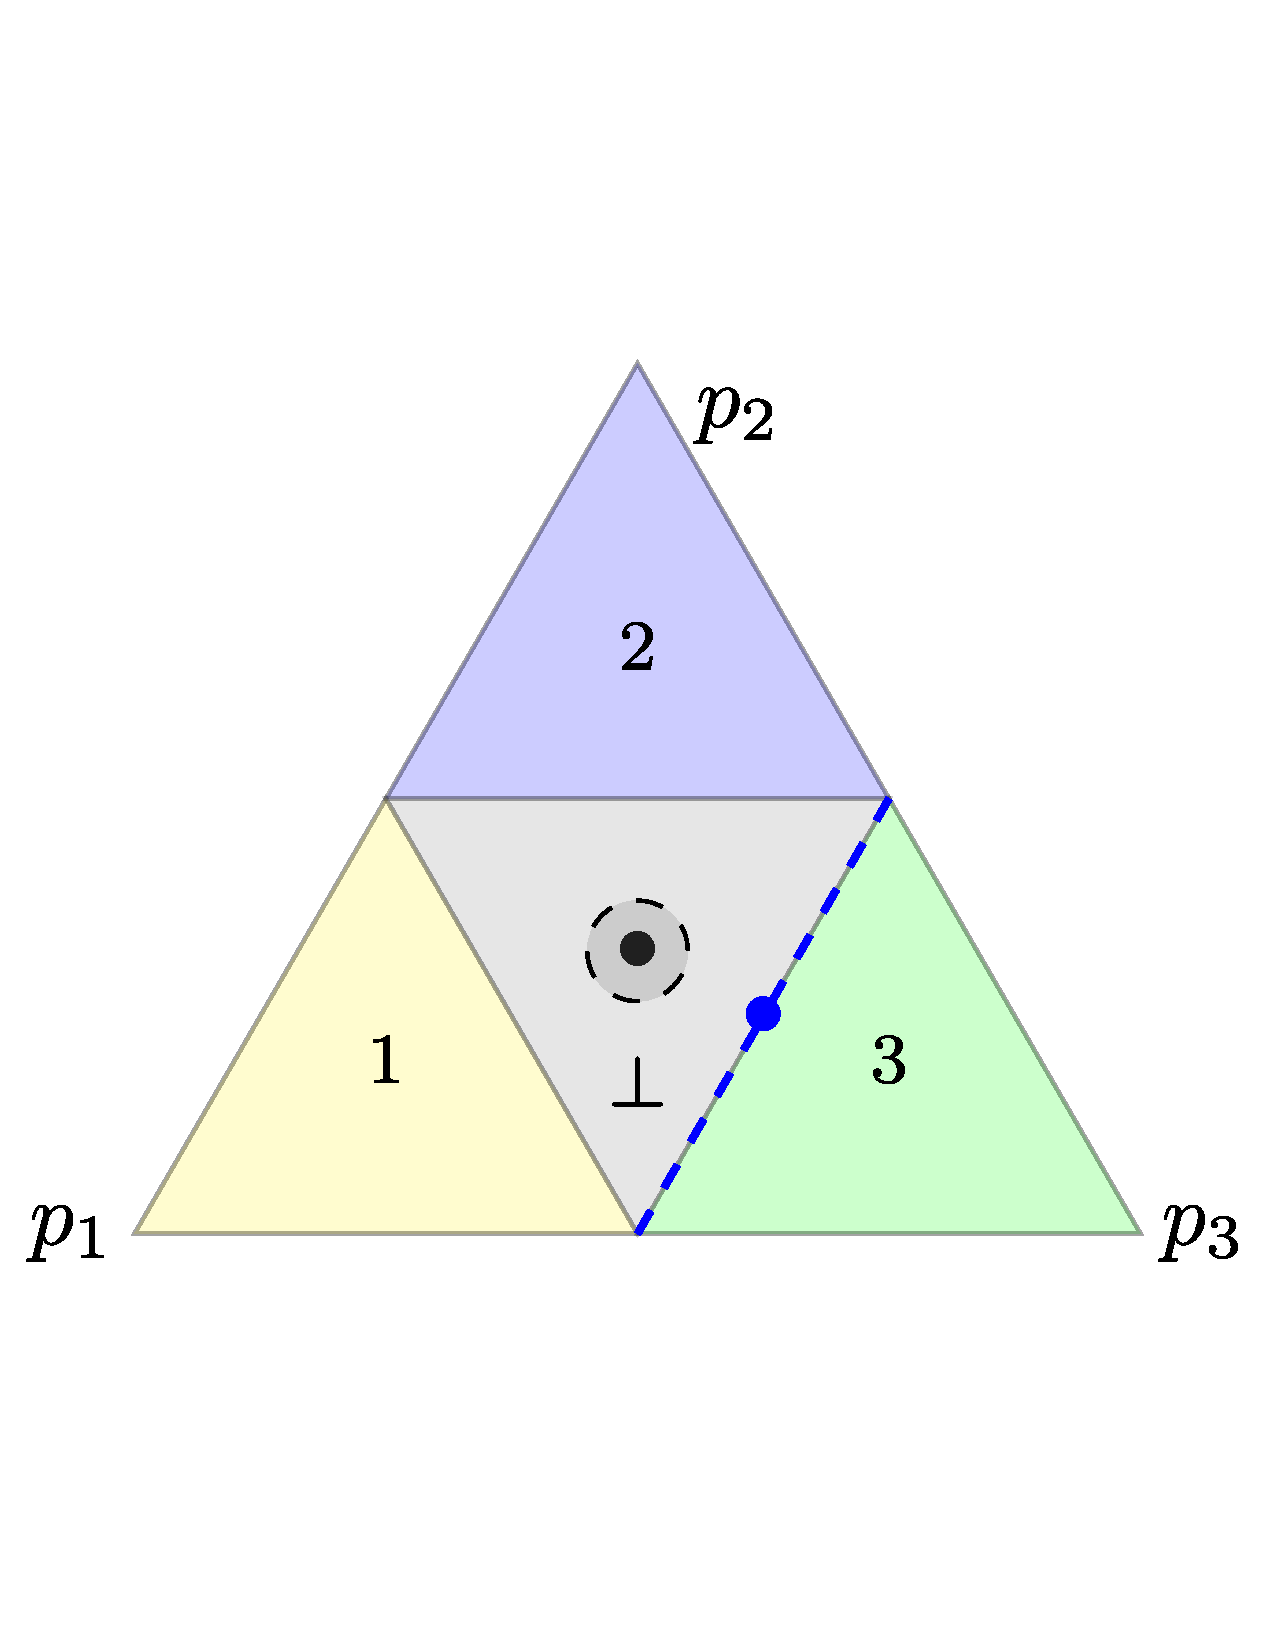
\includegraphics[width=\linewidth]{tikz/fsd-bound.pdf}
	\caption{Since the uniform distribution is in the relative interior of the simplex and the level set $\gamma_\bot$, its feasible subspace dimension is $2$. The distribution $(1/4, 1/4, 1/2)$, blue dot, has FSD $1$.}
	\label{fig:fsd-bound}
\end{minipage}
\hfill
\begin{minipage}{0.4\linewidth}
	\centering
	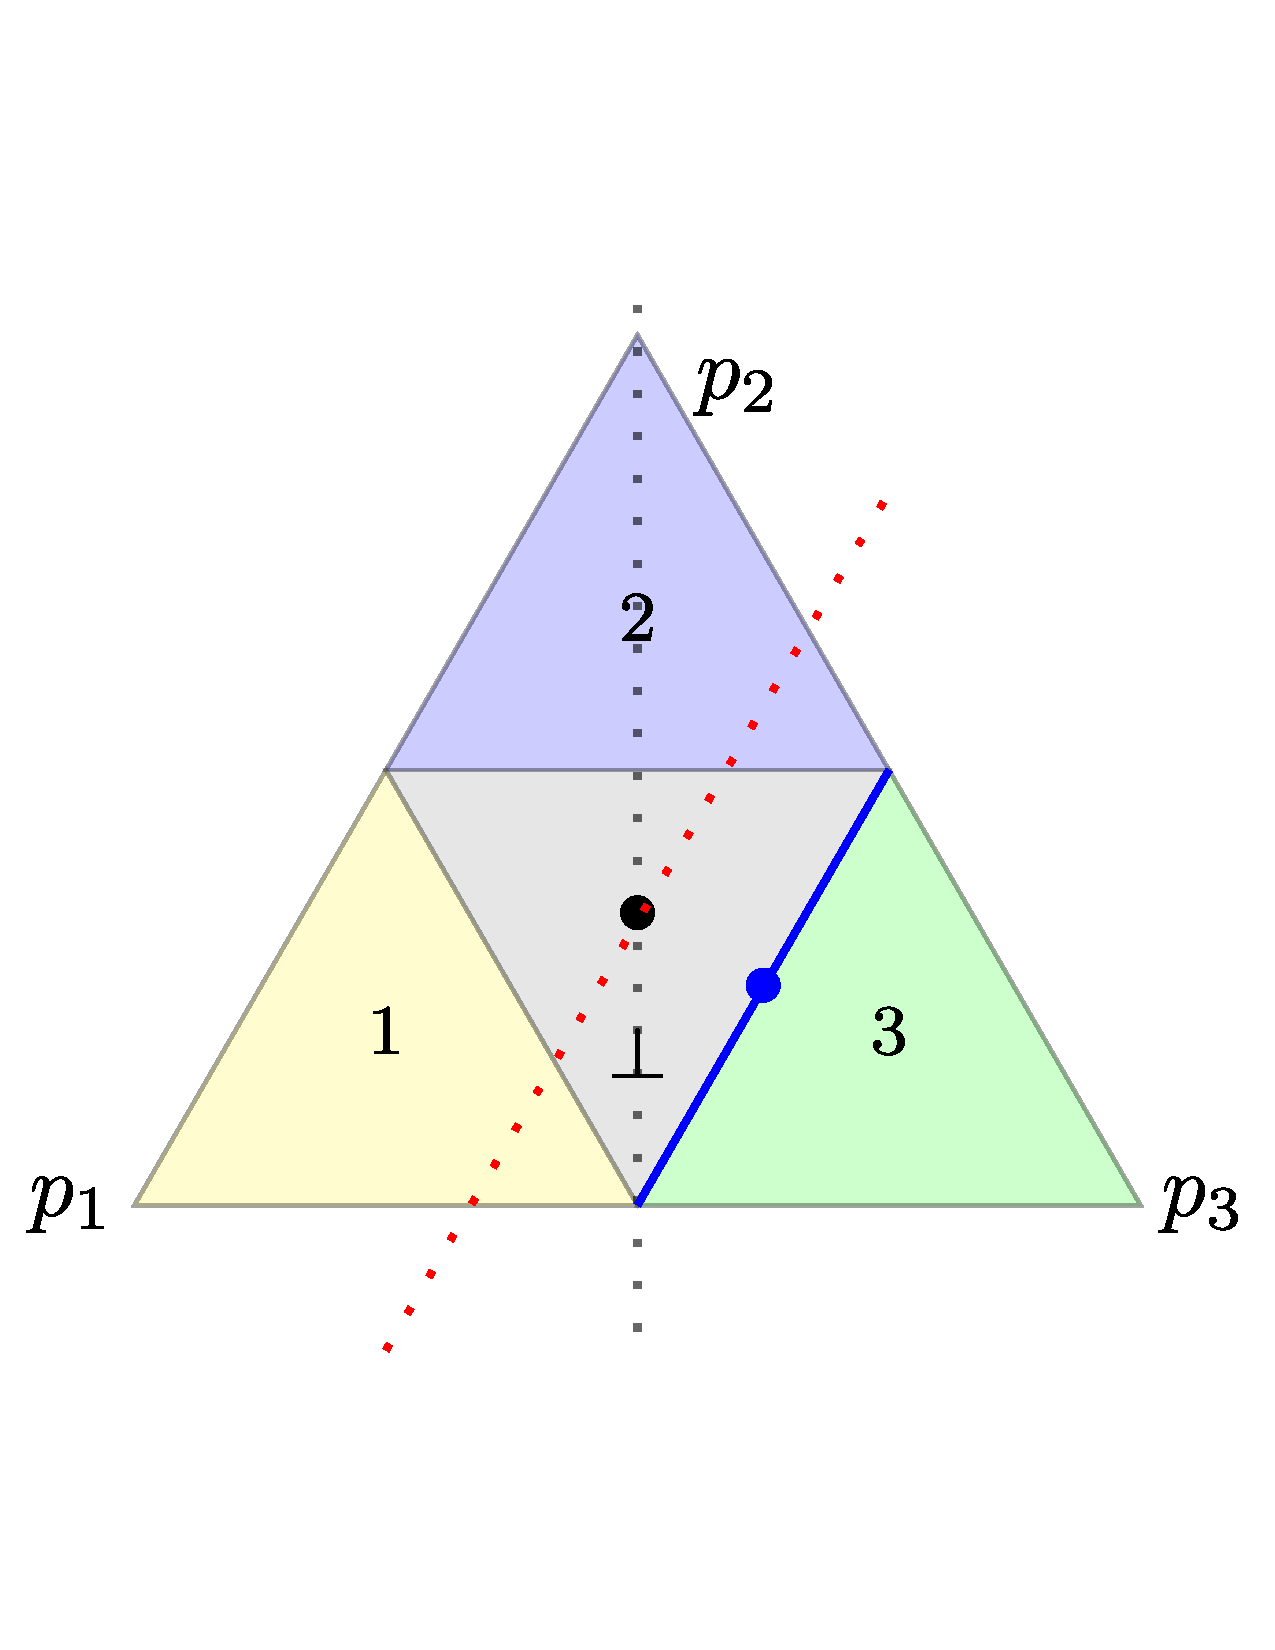
\includegraphics[width=\linewidth]{tikz/flats-bound.pdf}
	\caption{Any flat of codimension $1$ through the uniform distribution also leaves the (gray) cell $\gamma_\bot$ in the simplex. %However, for the distribution $p = (1/4, 1/4, 1/2)$, there is a $1$ dimensional flat containing $p$ that is a subseteq of $\gamma_\bot$ and $\gamma_3$.
	}
	\label{fig:flats-bound}
\end{minipage}
\end{figure}

\section{Continuous-valued predictions}\label{sec:contin-consis}

%commented out Jun 1 2020
%Theorem~\ref{thm:consistent-implies-indir-elic} allows us to use convex elicitation complexity as a tool to understand efficiency of consistent convex surrogates for a given property, which is more often what is given in a continuous estimation setting.
%For example, when one wants to learn an $\alpha$-quantile, we start with the property rather than a loss.
%In the literature, pinball loss $L(r,y) = (r-y)(\ones_{r \geq y} - \alpha)$ typically appears without explanation or justification as to why it is relevant in relation to the $\alpha$-quantile.
%Elicitation teaches us why pinball loss is consistent for learning a quantile as the pinball loss elicits the $\alpha$-quantile.
In continuous estimation problems, often one does not start with a target loss per se, but instead with a conditional statistic of the data one wishes to estimate, such as the conditional mean, variance, or entropy.
In this setting, Theorem~\ref{thm:cvx-flats} gives lower bounds on the prediction dimension of convex losses with a link to the desired conditional statistic, i.e., the convex elicitation complexity.
In particular, following an argument from~\citet{frongillo2018elicitation}, below Theorem~\ref{thm:bayes-risk-lower-bound} yields new bounds on the convex elicitation complexity of properties quantifying risk or uncertainty such as variance and entropy.
These bounds address an open question posed by~\citet{frongillo2018elicitation}, that of developing a theory of elicitation complexity for convex losses;
\raft{for cts pred}
our results show that not only is this theory possible, but the bounds thus far remain the same for convex losses.
\raft{complexity wrt surrogates they consider}
\botodo{I didn't understand this precisely -- ``bounds remain the same for convex losses''. Can we phrase this more precisely/accurately? Also, should we mention 2agarwal here?}\jessiet{To my understanding: elicitation complexity of variance and entropy (which are identifiable) = convex elicitation complexity of var and entropy}
Extending to infinite $\Y$, such as $\Y=\reals$, remains open.


% Theorem~\ref{thm:cvx-flats} also addresses one major open question  from~\citet{frongillo2015elicitation,frongillo2018elicitation}\jessiet{which citation?}: \emph{what are lower bounds on convex elicitation complexity?}
% While Theorem~\ref{thm:cvx-flats} is a statement about consistent surrogates, the heart of it is actually about indirect property elicitation.
% Thus, the result also applies to extend previous results~\citep{frongillo2015elicitation,frongillo2018elicitation} to provide new bounds on elicitation complexity for certain classes of properties in Theorem~\ref{thm:bayes-risk-lower-bound}.


% When extending the results of~\cite{frongillo2018elicitation}, we assume a property is identifiable, meaning its level sets are flats.
% \begin{definition}
%   A property $\Gamma:\simplex\to\R$ is \emph{$d$-identifiable} if its level sets are flats of co-dimension at most $d$ intersected with $\simplex$.
%   We write $\iden(\Gamma) = \min\{d \in \mathbb{N} : \Gamma\text{ is $d$-identifiable}\}$.
% \end{definition}

In the proof of Theorem~\ref{thm:bayes-risk-lower-bound} below, we modify the argument of~\citet[Corollary 7]{frongillo2018elicitation} to bound the convex elicitation complexity of the Bayes risk of the loss.
\raft{Note to self: need to sync the refs to the actual version on arxiv... or something...}
%\begin{restatable}{theorem}{bayesrisklowerbound}\label{thm:bayes-risk-lower-bound}
\begin{restatable}{theorem}{bayesrisklowerbound}\label{thm:bayes-risk-lower-bound}
  Let $L$ elicit some $\Gamma:\simplex\to\reals^d$.
  Let $p\in\relint\simplex$ and let $\Gamma_r$ be some level set of $\Gamma$ such that
  (i) $p\in\Gamma_r$,
  (ii) $\codim(\affhull(\Gamma_r))=d$, and
  (iii) either $\Gamma_r$ is a singleton or $\lbar$ is nonconstant on $\Gamma_r$.
  Then $\eliccvx(\lbar) \geq \min(d+1,n-1)$.
\end{restatable}

\begin{proof}[Proof sketch]
  To indirectly elicit $\lbar$, we must link from a loss $\hat L: \reals^k \times \Y \to \reals$.
  Using an argument of \citet[Theorem 4]{frongillo2018elicitation}, the property $\hat\Gamma = \prop{\hat L}$ refines $\Gamma$, in the sense that every level set of $\hat\Gamma$ is contained in a level set of $\Gamma$.
  If $\lbar$ is non-constant (the interesting case) on the level set $\Gamma_r$ containing $p$, then $\Gamma_r$ must strictly contain some level set $\hat \Gamma_{\hat r}$ containing $p$.
  But by Theorem 2, there is a flat $\hat{F}$ of small codimension, i.e. at most $k$, through $p$ yet strictly contained in $\affhull(\Gamma_r)$ (i.e. having strictly larger codimension).
  So $k \geq d + 1$.
\end{proof}


\paragraph{Example: Variance.}
As a warm-up, let us see how to show $\eliccvx(\Var)=2$ whenever $|\Y|\geq 3$, meaning the lowest dimension of a convex loss to estimate conditional variance is 2.
It is interesting to note that, to the best of our knowledge, even this simple bound is novel.
While intuitively obvious, the lower bound of 2 is not trivial.
In particular, the well-known fact that the variance is not elicitable does not yield this lower bound, as it does not rule out the variance being a link of a real-valued convex-elicitable property; cf.~\citet{frongillo2018elicitation}.

Let $\Y\subseteq\reals$ be a finite set with $n=|\Y|$.
Observe that the variance of $Y$ is the Bayes risk of squared loss $L(r,y) = (r-y)^2$; as $L$ elicits the mean $\Gamma(p) = \E_p Y$, we have $\Var_p[Y] = \E_p (\E_pY - Y)^2 = \min_{r\in\reals} \E_p L(r,Y)$.
To apply Theorem~\ref{thm:bayes-risk-lower-bound}, we take this $L$ and $\Gamma$ and $d=1$, and must choose an appropriate level set $\Gamma_r$; we choose $p = \tfrac 1 n \ones$ to be the uniform distribution and let $r=\E_pY$.
We summarize three conditions here, leaving the full details to Appendix~\ref{app:variance-example}:
(i) $p\in\Gamma_r$ by construction.
(ii) Letting $v\in\reals^\Y$ with $v_y = y - r$, the flat $F = \ker W \cap \affhull(\simplex)$ for $W = [v]\in\reals^{1\times n}$ contains $\Gamma_r$, and has $\codim(\affhull(\Gamma_r)) = \rank(W) = 1 = d$.
(iii)
$\Gamma_r=\{p\}$ is a singleton for $n \leq 2 = d+1$, and for $n\geq 3$ there are enough degrees of freedom in $\simplex$ for there to be two distributions with mean $r$ and different variances.

Applying Theorem~\ref{thm:bayes-risk-lower-bound} gives $\eliccvx(\Var) \geq \min(2,n-1)$, as desired.
In fact, this bound is tight for all $n$.
For $n=1$ there is only one distribution and we have complexity $0$; for $n=2$ the mean itself, elicited by squared loss, determines the distribution; for $n\geq 3$ we may elicit the first two moments via the convex $L(r,y) = (r_1-y)^2 + (r_2-y^2)^2$, and recover the variance via $\psi(r) = r_2-r_1^2$.

\paragraph{Example: Entropy and Norms.}
For another application, let us see how Theorem~\ref{thm:bayes-risk-lower-bound} implies $\eliccvx(G) = n-1$ for any strictly concave function $G:\simplex\to\reals$ of the distribution, including most entropy functions.
In other words, there is no convex loss function allowing one to consistently estimate conditional entropy using fewer dimensions than required to estimate the conditional distribution itself.
This observation also extends to norms; given any $k>1$, $G(p) = \|p\|_k^k$ is strictly convex, and hence $\eliccvx(\|\cdot\|_k) = n-1$, as otherwise we could link to $G$ via $\psi(r) = r^k$.
These results illustrate the power of our technique.

To show the bound, recall that $G$ is the Bayes risk of a proper loss defined by $L(p,y) = G(p) + s_p \cdot (\delta_y - p)$, where $\delta_y(y') = \ones\{y=y'\}$ is the point distribution on $y$ and $-s_p \in \partial (-G)(p)$ is a subgradient of $-G$ at $p$~\citep{gneiting2007strictly,reid2009surrogate,frongillo2014general}.
Intuitively, since $L$ elicits the identity property $\Gamma(p)=p$, Theorem~\ref{thm:bayes-risk-lower-bound} should therefore give us a maximal lower bound ($n-1$), as the level sets of are $\Gamma$ have codimension $n-1$.
For technical reasons, however, we need to drop a dimension from the prediction space, e.g.\ via the bijection $\varphi(p) = (p_1,\ldots,p_{n-1})$, defining $L'(p',y) = L(\varphi^{-1}(p'),y)$ which elicits $\Gamma'(p) = \varphi(p)$ but still has Bayes risk $G$.
Now the conditions of Theorem~\ref{thm:bayes-risk-lower-bound} are easily checked, where again $p\in\relint\simplex$ is the uniform distribution and $r=\varphi(p)$: (i) is trivial, (ii) $\codim(\affhull(\Gamma_r')) = \codim(\{p\}) = n-1$, and (iii) $\Gamma_r'$ is a singleton.
As with the variance example, the lower bound is easily matched, e.g.\ by $L_2(p',y) = \|\varphi^{-1}(p')-\delta_y\|_2^2$, which is convex in $p'$, and the link $\psi(p') = G(\varphi^{-1}(p'))$.


\section{Conclusions and future work}\label{sec:conclusions}
In this work, we show that indirect property elicitation can be studied as a necessary condition for the existence of a consistent surrogate loss (Theorem~\ref{thm:consistent-implies-indir-elic}).
Furthermore, we introduce a new lower bound (Theorem~\ref{thm:cvx-flats}) on the dimension of a consistent convex loss that is generally applicable and extends previous results from both the discrete prediction and continuous estimation settings.
Bounding the prediction dimension on convex surrogate losses may yield significant improvements in the complexity of the optimization algorithm as a whole.

While this work tightens bounds on the dimension of consistent surrogate losses, it does not completely characterize the dimensionality of a convex surrogate for a given problem.
One might be able to further tighten these bounds by property elicitation by studying monotonicity and adjacency of level sets.
In discrete predictions, these bounds might also be tightened if the equivalence of convex calibration dimension and embedding dimension of~\citet{finocchiaro2020embedding} is shown; the current embedding dimension bounds are not tight either, but additional structure is imposed by considering the embedding framework.
Moreover, the practical reason why consistency is desired is to ensure the guarantee of empirical risk minimization (ERM) rates; however, the relationship between ERM rates and property elicitation has not been studied.
Lastly, Theorem~\ref{thm:cvx-flats} relies on Minkowski sums, which have not been clearly defined for infinite $\Y$; we leave this generalization as an open question.
\btw{Infinite losses/minnable restriction}
\btw{two questions: 1. if dim d loss works, does dim d minnable loss work? 2. would defining rays as part of the support space work?}

\newpage

\section*{Broader Impact}
This work is entirely theoretical, thus the opportunity for broader impacts is indirect, but still present.
Understanding the complexity and efficiency of consistent, convex surrogates for different target losses and properties we wish to learn can lead to understanding the tradeoffs that are often made in ad-hoc surrogates that are not consistent.
These ad-hoc surrogates are consistent with respect to \emph{some property}, although it may not be the one we wish to elicit, either directly or indirectly.
As a general prediction task arises, one might be able to use property elicitation to understand what question they are actually answering (in the best base, with sufficient data that matches the real-world data distribution) by minimizing their surrogate loss and how it differs from the question they are actually trying to answer.

\begin{ack}
Nishant, Adam
\end{ack}

\bibliographystyle{plainnat}
\bibliography{diss,extra}

\newpage
\appendix
\section{A general notion of calibration}\label{app:calibration}
For general settings, we introduce a new notion of calibration that is a special case of calibration as introduced by~\citet[Chapter 3]{steinwart2008support}.
We will show that in discrete prediction settings, it is equivalent to the more commonplace definition given in Definition~\ref{def:calibrated-finite}.
Therefore, we use this more general definition of calibration when proving statements about the relationship between consistency, calibration, and indirect elicitation.

\begin{definition}[Calibrated]\label{def:calibrated-general}
	A loss $L:\reals^d \times \Y \to \reals$ is \emph{calibrated} with respect to a loss $\ell : \R \times \Y \to \reals$ eliciting the property $\gamma$ if there is a link $\psi : \reals^d \to \R$ such that, for all distributions $p \in \simplex$, there exists a function $\zeta : \reals_+ \to \reals_+$ with $\zeta$ continuous at $0^+$ and $\zeta(0) = 0$ such that for all $u \in \reals^d$, we have
	\begin{equation}\label{eq:calibrated-general}
	\ell( \psi(u); p) - \risk{\ell}(p)  \leq \zeta \left(  \exploss{L}{u}{p} - \risk{L}(p) \right)~.~
	\end{equation}
\end{definition}

Consider the following four conditions: Suppose we are given $\zeta:\reals_+ \to \reals_+$.
\begin{enumerate}
	\item [A] $\zeta$ satisfies $\zeta : 0 \mapsto 0$ and is continuous at $0$.
	\item [B] $\epsilon_m \to 0 \implies \zeta(\epsilon_m) \to 0$.
	\item [C] Given $\zeta:\reals \to \reals_+$, for all $u \in \reals^d$, $R_\ell(\psi(u); p) \leq \zeta(R_L(u;p))$.
	\item [D] For all $p \in \simplex$ and sequences $\{u_m\}$ so that $R_L(u_m; p) \to 0$, we have $R_\ell(\psi(u_m); p) \to 0$.
\end{enumerate}
The existence of a function $\zeta$ so that $(A \wedge C)$ defines calibration as in Definition~\ref{def:calibrated-general}, and we show $A \iff B$ in Lemma~\ref{lem:continuous-iff-limits}.  
Lemma~\ref{lem:calib-converging-regrets} shows calibration if and only if $D$, which yields a condition equivalent to calibration without dependence the function $\zeta$.

\begin{proposition}
	When $\R$ is finite, a continuous loss and link $(L, \psi)$ are calibrated with respect to a target loss $\ell$ via Definition~\ref{def:calibrated-general} if and only if calibration via Definition~\ref{def:calibrated-finite}.
\end{proposition}\jessiet{Okay if $\Gamma$ is empty}
\begin{proof}
$\implies$
	We prove the contrapositive; if $(L, \psi)$ is not calibrated with respect to $\ell$ by Definition~\ref{def:calibrated-finite}, then it is not calibrated via Definition~\ref{def:calibrated-general} either.
	If $(L, \psi)$ are not calibrated with respect to $\ell$ by Definition~\ref{def:calibrated-finite}, then there is a $p \in \simplex$ so that $\inf_{u : \psi(u) \not \in \gamma(p)} \exploss{L}{u}{p} = \inf_u \exploss{L}{u}{p}$.
	Thus there is a sequence $\{u_m\}$ so that $\lim_{m \to \infty} \psi(u_m) \not \in \gamma(p)$ and $\exploss{L}{u_m}{p} \to \risk{L}(p)$.  
	Now we have $R_L(u_m; p) \to 0$ but $R_\ell(\psi(u_m); p) \not \to 0$, so by Lemma~\ref{lem:calib-converging-regrets}, we contradict calibration by Definition~\ref{def:calibrated-general}.
%	
% Commented out 05.19.2020 for easier proof if Lemma 5 is true.
%	We prove the contrapositive; if $(L, \psi)$ is not calibrated with respect to $\ell$ by Definition~\ref{def:calibrated-finite}, then it is not calibrated via Definition~\ref{def:calibrated-general} either.
%	
%	Suppose there was a distribution $p \in \simplex$ so that $\inf_{u : \psi(u) \not \in \gamma(p)} L(u;p) = \inf_{u} L(u;p)$.
%	There must then be a sequence $\{u_m\} \to u$ so that $\lim_{m \to \infty} \psi(u_m) \not \in \gamma(p)$ and $L(u_m; p) \to \risk{L}(p)$.
%	
%	This consequently implies $R_L(u_m;p) \to 0$ as $L(u_m; p) \to \risk{L}(p)$, but as $\ell(\psi(u_m); p) \not \to \risk{\ell}(p)$ (if it did converge, then we would have $\psi(u_m) \to r \in \gamma(p)$), so $R_\ell(\psi(u_m); p) \not \to 0$.
%	Thus, by Lemma~\ref{lem:calib-converging-regrets}, we have no calibration via Definition~\ref{def:calibrated-general}.  

$\impliedby$
Suppose there was a function $\zeta$ satisfying the bound in Equation~\eqref{eq:calibrated-general} for a fixed distribution $p \in \simplex$.
Observe the bound in Equation~\eqref{eq:calibration} can be written as $R_L(u,p) > 0$ for all $p \in \simplex$ and $u$ such that $\psi(u)$ is bounded away from $\gamma(p)$. \jessie{details correct??}

By Equation~\eqref{eq:calibrated-general}, for any sequence $\{u_m\}$ so that $\psi(u_m) \not \to \gamma(p)$, we have must have $\zeta(R_\ell(\psi(u_m), p)) \not \to 0$ as we would otherwise contradict the bound in Equation~\eqref{eq:calibrated-general} since $R_\ell(\psi(u), p) \not \to 0$. 
Therefore $R_L(u_m, p) \not \to 0$; thus, the strict inequality holds.
\end{proof}

The following Lemma shows that conditions $A$ and $B$ are equivalent, so that we can using condition $B$ in lieu of condition $A$ in the proof of Lemma~\ref{lem:calib-converging-regrets}
\begin{lemma}\label{lem:continuous-iff-limits}
	A function $\zeta:\reals \to \reals$ is continuous at $0$ and $\zeta(0) = 0$ if and only if the sequence $\{u_m\} \to 0 \implies \zeta(u_m) \to 0$.
	\jessie{$A \iff B$}
\end{lemma}
\begin{proof}
	$\implies$ Suppose we have a sequence $\{u_m\} \to 0$.
	By continuity, we have $\lim_{u_m \to 0}\zeta(u_m) = \zeta(0) = 0$, so $\zeta(u_m) \to 0$.
	
	$\impliedby$ Suppose $\zeta(0) \neq 0$ but $\zeta$ was continuous at $0$.
	The constant sequence $\{u_m\} = 0$ then converges to $0$, but as $\zeta$ is continuous at $0$, we must have $\lim_{m \to \infty}\zeta(u_m) = \zeta(0) \neq 0$, so $\zeta(u_m) \not \to 0$.
	
	Now suppose $\zeta(0) = 0$ but $\zeta$ was not continuous at $0$.
	There must be a sequence $\{u_m\} \to 0$ so that $\lim_{m \to \infty}\zeta(u_m) \neq \zeta(0) = 0$, so $\zeta(u_m) \not \to 0$.
\end{proof}

Lemma~\ref{lem:calib-converging-regrets} now gives a condition equivalent to calibration without requiring one to already have a function $\zeta$ in mind.
\begin{lemma}\label{lem:calib-converging-regrets}
	A continuous surrogate and link $(L,\psi)$ are calibrated (via definition~\ref{def:calibrated-general}) with respect to $\ell$ if and only if, for all $p \in \simplex$ and sequences $\{u_m\}$ so that $R_L(u_m; p) \to 0$, we have $R_\ell(\psi(u_m); p) \to 0$.
	\jessie{$(A \wedge C) \iff D$}
\end{lemma}
\begin{proof}
\jessie{$(A \wedge C) \implies D$}
	$\implies$ Take a sequence $\{u_m\}$ so that $R_L(u_m;p) \to 0$.
	Since $\zeta(0) = 0$ and $\zeta$ is continuous at $0$, we have $\zeta(R_L(u_m;p)) \to 0$.
	As the bound from Equation~\eqref{eq:calibrated-general} is satisfied for all $u \in \reals^d$ by assumption, we observe
	\begin{align*}
	\forall m, \; &0 \leq R_\ell(\psi(u_m); p) \leq \zeta(R_L(u_m;p))\\
	\implies &0 \leq \lim_{m \to \infty} R_\ell(\psi(u_m); p) \leq \lim_{m \to \infty} \zeta(R_L(u_m;p)) = 0\\
	\implies &0 = \lim_{m\to\infty} R_\ell(\psi(u_m); p) ~.~
	\end{align*}
	
	
	$\impliedby$ 
\jessie{$D \implies (A \wedge C)$}
	Fix $p \in \simplex$, and consider $\zeta(c) := \sup_{u: R_L(u,p) \leq c} R_\ell(\psi(u); p)$.  
	We will show $R_L(u_m; p) \to 0 \implies R_\ell(\psi(u_m); p) \to 0$ gives calibration via the function $\zeta$ constructed above. 
	With $\zeta$ as constructed, we observe that the bound in equation~\eqref{eq:calibrated-general} is satisfied for all $u \in \reals^d$ and apply Lemma~\ref{lem:continuous-iff-limits} to observe that if there is a sequence $\{\epsilon_m\} \to 0$ so that $\zeta(\epsilon_m) \not \to 0$, it is because $R_L(u_m, p) \not \to 0 \not\implies R_\ell(\psi(u_m), p) \to 0$.
	

\jessie{D $\implies$ C}
Now, we observe that the bound in Equation~\eqref{eq:calibrated-general} is satisfied for all $u \in \reals^d$ by construction of $\zeta$.
Let $S(v) := \{u' \in \reals^d : R_L(u';p) \leq R_L(v,p) \}$.
Showing $R_\ell(\psi(u);p) \leq \sup_{u' \in S(u)} R_\ell(\psi(u') ; p)$ for all $u \in \reals^d$ gives the condition $C$.
As $u$ is in the space over which the surpremum is being taken (as $R_L(u;p) \leq R_L(u;p)$), we then have calibration by definition of the supremum.

\jessie{Not $B$ leads to contradiction of $D$.}
Now suppose there exists a sequence $\{\epsilon_m\} \to 0$ so that $\zeta(\epsilon_m) \not \to 0$.
Consider $S(\epsilon) = \{u \in \reals^d : R_L(u,p) \leq \epsilon\}$.

\begin{align*}
\epsilon_1 \leq \epsilon_2 &\implies S(\epsilon_1) \subseteq S(\epsilon_2)\\
&\implies \zeta(\epsilon_1) \leq \zeta(\epsilon_2)~.~
\end{align*}
Now suppose there exists a sequence $\{u_m\}$ so that $R_L(u_m, p) \to 0$.
Then for all $\epsilon > 0$, there exists a $m' \in \mathbb{N}$ so that $R_L(u_m, p) < \epsilon$ for all $m \geq m'$.
Since this is true for all $\epsilon$, we have $S(\epsilon)$ nonempty for all $\epsilon > 0$, and therefore $\zeta(c)$ is discrete for all $c > 0$.
Now if $\zeta(\epsilon_m) \not \to 0$, it must be because $R_\ell(\psi(u_m), p) \not \to 0$ for some sequence converging to zero surrogate regret, and therefore we contradict the statement $R_L(u_m, p) \to 0 \implies R_\ell(\psi(u_m), p) \to 0$.

Moreover, we argue that such a sequence of $\{u_m\}$ with converging surrogate regret always exists by continuity and boundedness from below of the surrogate loss,
\btw{really just need lower semi-continuity and boundedness from below}
since we can take the constant sequence at the (attained) infimum.
%
%\jessie{$D \implies A$, but actually $\lnot B \wedge C \implies \lnot D$}
%Fix $p \in \simplex$.
%Suppose we have a sequence $\{\epsilon_m\}$ so that $\epsilon_m \to 0$, but $\zeta(\epsilon_m) \not \to 0$.
%If $L$ is continuous over the reals \jessiet{Need this, right?}, then for each $m$, we can construct a subsequence $\{u^j_m\}$ so that $R_L(u^j_m, p) \to \epsilon_m$ for all $m$.
%We can now construct the sequence $\{\epsilon'_m\}$ with $\epsilon'_m = \lim_{j \to \infty} R_L(u^j_m, p)$.
%This sequence converges to $0$, but we have $\lim_{m \to \infty} \zeta(\epsilon'_m) = \lim_{m \to \infty} \lim_{j \to \infty} \zeta(R_L(u^j_m, p)) \not \to 0$. 
%As $R_\ell(\psi(u_m); p) \leq R_L(u_m; p)$ for all $m$, we then have this being true in the limit.
%For this sequence, this then gives a loose bound of $0 \leq \lim_{m\to\infty} R_\ell(\psi(u_m); p) \leq c$. 
%	
\end{proof}

\subsection{Relating calibration, consistency, and indirect elicitation.}
Even with the more general notion of calibration that extends beyond discrete predictions, we still have consistency implying calibration.
\begin{proposition}\label{prop:consistent-implies-calibrated}
	If a loss and link $(L, \psi)$ are consistent with respect to a loss $\ell$, then they are calibrated with respect to $\ell$.
\end{proposition}
\begin{proof}
	We show the contrapositive.
	If $(L, \psi)$ are not calibrated with respect to $\ell$, then there is a sequence $\{u_m\}$ such that $R_L(u_m; p) \to 0$ but $R_\ell(\psi(u_m); p) \not \to 0$ via Lemma~\ref{lem:calib-converging-regrets}.
	Suppose $D \sim \X \times\Y$ has only one $x \in \X$ with $Pr_D(X = x) > 0$ so that $p := D_x$ and $\E_D f(X,Y) = \E_p f(x, Y)$.
	Consider any sequence of functions $\{f_m\} \to f$ with $f_m(x) = u_m$ for all $f_m$.
	Now we have $\E_D L(f_m(X), Y) \to \inf_f \E_D L(f(X), Y)$, but $\E_D \ell(\psi \circ f(X), Y) \not \to \inf_f \E_D \ell(\psi \circ f(X), Y)$, and therefore $(L, \psi)$ is not calibrated with respect to $\ell$.
\end{proof}

Moreover, we have calibration implying indirect elicitation.
\begin{lemma}\label{lem:calib-implies-indir}
	If a surrogate and link $(L, \psi)$ are calibrated with respect to a loss $\ell:\R \times\Y \to \reals$, then $L$ indirectly elicits the property $\gamma := \prop{\ell}$.
\end{lemma}
\begin{proof}
	Let $\Gamma$ be the unique property directly elicited by $L$, and fix $p \in \simplex$ with $u$ such that $p \in \Gamma_u$.
  \raft{Use $\Gamma(p) \neq \emptyset$ here!}
	As $p \in \Gamma_u$, then $\zeta(\exploss{L}{u}{p} - \risk{L}(p)) = \zeta(0) = 0$, we observe the bound $\ell(\psi(u); p) \leq \risk{\ell}(p)$.
	We also have $\ell(\psi(u); p) \geq \risk{\ell}(p)$ by definition of $\risk{\ell}$, so we must have $\ell(\psi(u);p) = \risk{\ell}(p) = \ell(\gamma(p); p)$, and therefore, $p \in \gamma_{\psi(u)}$.
	Thus, we have $\Gamma_u \subseteq \gamma_{\psi(u)}$, so $L$ indirectly elicits $\gamma$.
\end{proof}

Combining the two results, we can observe the result of Theorem~\ref{thm:consistent-implies-indir-elic} another way: \emph{through calibration}.

\section{Omitted Proofs}\label{app:omitted-proofs}

\subsection{Coping with links for elicitable set-valued properties}
A hyperplane weakly separates two sets if its two closed halfspaces respectively contain the two sets.
\begin{lemma}\label{lem:intersect-levelsets}
	If $\gamma: \simplex \toto \R$ is an elicitable property, then for any pair of predictions $r, r' \in \R$ where $\gamma_r \neq \gamma_{r'}$, there is a hyperplane $H = \{x \in \reals^{\Y} : v \cdot x = 0\}$, for some $v \in \reals^\Y$, that weakly separates $\gamma_r$ and $\gamma_{r'}$ and has $\gamma_r \cap H = \gamma_{r'} \cap H = \gamma_r \cap \gamma_{r'}$.
\end{lemma}
\begin{proof}
	\btw{Bo: the proof holds as written for the case where the level sets have empty intersection.}
	Let $\ell$ elicit $\gamma$.
	Let $v = \ell(r, \cdot) - \ell(r', \cdot)$, interpreted as a nonzero vector in $\reals^\Y$.
	Let $H = \{ q : v \cdot q = 0 \}$.
	If $v \cdot q < 0$, then $r'$ cannot be optimal, so $q \not\in \gamma_{r'}$.
	So $\gamma_{r'} \subseteq \{ q : v \cdot q \geq 0 \}$.
	Symmetrically, $\gamma_r \subseteq \{ q : v \cdot q \leq 0 \}$.
	This is weak separation, and it immediately implies that $\gamma_r \cap \gamma_{r'} \subseteq H$.
	
	Finally, if and only if $v \cdot q = 0$, i.e. $q \in H$, by definition the expected losses of both reports are the same.
	So $q \in \gamma_r \cap H \iff q \in \gamma_{r'} \cap H$.
	This gives $\gamma_r \cap H = \gamma_{r'} \cap H = \gamma_r \cap \gamma_{r'} \cap H = \gamma_r \cap \gamma_{r'}$.
\end{proof}

\begin{lemma}\label{lem:set-valued-prop-flats}
	Suppose we are given an elicitable property $\gamma : \simplex \toto \R$ and distribution $p \in \relint\simplex$ such that $p \in \gamma_r \cap \gamma_{r'}$ for $r,r' \in \R$.
	Then for any flat $F$ containing $p$, $F \cap \simplex \subseteq \gamma_r \iff F \cap \simplex \subseteq \gamma_{r'}$.
\end{lemma}
\begin{proof}
	If $\gamma_r = \gamma_{r'}$, we are done.
	Otherwise, Lemma \ref{lem:intersect-levelsets} gives a hyperplane $H = \{ x \in \reals^\Y : v \cdot x = 0\}$ and a guarantee that $\gamma_r \subseteq \{ q \in \simplex : v \cdot q \leq 0\}$, while $\gamma_{r'} \subseteq \{ q \in \simplex : v \cdot q \geq 0 \}$, and finally $\gamma_r \cap \gamma_{r'} \subseteq H$.
	
	Suppose $F \cap \simplex \subseteq \gamma_r$.
	We show $F \cap \simplex \subseteq \gamma_{r'}$.
	Let $q \in F \cap \simplex$.
	We claim that for small enough $\epsilon$, the point $q' = p - \epsilon (q-p)$ is in $F \cap \simplex$ as well.
	Containment in $F$ follows because both $p$ and $q$ are in $F$ and it is a flat, while containment in $\simplex$ follows because $p \in \relint\simplex$.
	
	Now, suppose for contradiction that $q \not\in \gamma_{r'}$.
	Then $v \cdot q < 0$: containment in $\gamma_r$ gives $v \cdot q \leq 0$, and if $v \cdot q = 0$ then $q \in \gamma_r \cap H \implies q \in \gamma_{r'}$, a contradiction.
	But, noting that $p \in H$, we have $v \cdot q' = -\epsilon (v \cdot q) > 0$, so $q'$ is not in $\gamma_{r}$.
	This contradicts the assumption $F \cap \simplex \subseteq \gamma_r$.
	Therefore, we must have $q \in \gamma_{r'}$, so we have shown $F \cap \simplex \subseteq \gamma_{r'}$.
	Because $r$ and $r'$ were completely symmetric, this completes the proof.
\end{proof}

\subsection{Reconstructing the result of~\citet[Theorem 16]{ramaswamy2016convex}}
\begin{lemma}\label{lem:feas-sub-is-a-flat}
	Suppose we have the discrete elicitable property $\gamma$ and distribution $p \in \relint{\simplex}$ with $r \in \gamma(p)$.
	If $F$ is a flat in $\affhull(\simplex)$ containing $p$ such that $F \cap \simplex \subseteq \gamma_r$, then $F - p$ is a subspace contained in $\Sc_{\gamma_r}(p)$.
	%  \raf{I think you want $p$ in the interior of the simplex for now}
\end{lemma}
\begin{proof}
	Observe $F-p$ is a subspace as it is a linear shift of $F$, which is a linear subspace by definition of a flat and the fact that it contains $\vec 0$.
	Now consider $v \in F - p$.
	Since $p \in \relint{\simplex}$, there is an open ball of radius $\epsilon$ in the affine hull of $\simplex$ so that for all $q \in B(p, \epsilon)$, we have $q \in \simplex$.
	In particular, take $\alpha = \epsilon / 2$, and we observe $p \pm \alpha v \in B(p, \epsilon)$, and therefore $p \pm \alpha v \in \simplex$.
	Moreover, by the assumption $v \in F - p$, we also have $p \pm \alpha v \in \gamma_r$. 
	Since level sets of elicitable properties are convex (\citep{lambert2009eliciting}) this is true for all $\alpha' \leq \alpha$.
	Therefore, we observe $v \in S_{\gamma_r}(p)$, so $F-p \subseteq S_{\gamma_r}(p)$.
	%  First, if $p+v \in \gamma_r$ and $p -v \in \gamma_r$, then we have $v \in \Sc_{\gamma_r}(p)$ with $\epsilon_0 = 1$ as level sets of elicitable properties are convex by~\cite{lambert2009eliciting}.
	%  If either $p + v$ or $p - v \not \in \gamma_r$, it must be because the term is out of the simplex by definition of $F$.
	%  
	%  However, if both $p + \alpha^+ v$ and $p - \alpha^- v \in \simplex$ for some $\alpha^\pm \in (0,1)$, then $v \in \Sc_{\gamma_r}(p)$ with $\epsilon_0 = \min(\alpha^+, \alpha^-)$.
	%  As $p \in \relint{\simplex}$, there is always such an $\epsilon_0$; if there were not, then we would observe $v \not \in F - p$.
	%  Therefore, we have $v \in F - p \implies v \in \Sc_{\gamma_r}(p)$, so $(F - p) \subseteq \Sc_{\gamma_r}(p)$.
\end{proof}

The next result helps us generalize Lemma~\ref{lem:feas-sub-is-a-flat} to any $p$; not just to $p \in \relint{\simplex}$.
\newcommand{\simplexp}{\Delta_{\Y'}}
\begin{lemma}\label{lem:p-boundary-fsd}
	For any $p \in \simplex$ and $r$ such that $p \in \gamma_r$, take $\Y' := \supp(p)$.
	Define $\gamma' : \simplex \toto \R$ with $\gamma' : q \mapsto \gamma(q) \cap \simplexp$.
	Then $\dim(\Sc_{\gamma_r}(p)) = \dim(\Sc_{\gamma'_r}(p))$.
\end{lemma}
\begin{proof}
	Consider the ambient space of both $\Sc_{\gamma_r}(p)$ and $\Sc_{\gamma'_r}(p)$ is $\reals^\Y$.
	We trivially have $\dim(\Sc_{\gamma_r}(p)) \geq \dim(\Sc_{\gamma'_r}(p))$ since $\gamma'$ is simply $\gamma$ projected down to an affine subspace of $\reals^\Y$.
	
	Now to see $\dim(\Sc_{\gamma_r}(p)) \leq \dim(\Sc_{\gamma'_r}(p))$, it suffices to show subset inclusion.
	Take some $v \not \in \Sc_{\gamma'_r}(p)$.
	Observe that $\gamma'_r = \gamma_r \cap \simplexp$, so if $q^\pm := p \pm \epsilon v \not \in \gamma'_r$ for all $\epsilon > 0$, it is either because one of $q^+$ or $q^-$ is not in $\gamma_r$ or because either $q^\pm \not \in \simplexp$.
	The first case can be seen easily by the definition of $\gamma'$, and the latter can be seen because leaving $\simplexp$ means one of $q^\pm$ also is not in $\simplex$, and therefore not in $\gamma_r$ as $\gamma_r \subseteq \simplex$.
	Thus $\Sc_{\gamma_r}(p) = \Sc_{\gamma'_r}(p)$.
	%commented out 05.26.2020
	%	For simplicity, consider $\epsilon = \epsilon_0 / 2$.
	%	Consider $P := \spn(\{e_y : y \in \supp(p) \})$.
	%	\begin{align*}
	%	\dim(\Sc'_{\gamma_r}(p)) &= \dim(\Sc_{\gamma_r}(p)) + \dim(P) - \dim(\Sc_{\gamma_r}(p) + P)
	%	\end{align*}
	%	If $\dim(P) = \dim(\Sc_{\gamma_r}(p) + P)$, the claim holds.
	%	Be definition of $P$, we know $\dim(P) = \|p\|_0$, so we can show $\dim(\Sc_{\gamma_r}(p) + P) = \|p\|_0$.		
	%	One way to do this is to show $\Sc_{\gamma_r}(p) \subseteq P$.
	%	
	%	Suppose there was some $v \not\in P$ such that $v \in \Sc_{\gamma_r}(p)$.
	%	That means there is some $i$ so that $i \not \in \supp(p)$ (i.e. $p_i = 0$) but $v_i \neq 0$. \jessiet{Check this line.}
	%	However, if $v \in \Sc_{\gamma_r}(p)$, then there is some $\epsilon_0 > 0$ so that $p + \epsilon v$ and $p - \epsilon v \in \gamma_r \subseteq \simplex$ for all $\epsilon \in (0, \epsilon_0)$.
	%	For simplicity, consider $\epsilon = \epsilon_0 / 2$.
	%	Since $p_i = 0$, this gives $(p+\epsilon v)_i = (\epsilon v)_i$, and likewise for $(p - \epsilon v)_i$.
	%	As neither $\epsilon$ nor $v_i$ are $0$, one of these terms must be negative, and therefore not in the simplex.
	%	As $\gamma_r \subseteq \simplex$, we then have $v \not \in \Sc_{\gamma_r}(p)$.
	%	Therefore, $\Sc_{\gamma_r}(p) \subseteq P$, and $\dim(\Sc_{\gamma_r}(p) + P) = \dim(P) = \|p\|_0$.
\end{proof}

\hariresult*
\begin{proof}
	Let $L : \reals^d \times \Y \to \reals$ be a calibrated surrogate for $\ell$, and consider $\Y' := \supp(p)$ and what happens when we restrict $L$ and $\ell$ to only the outcomes in $\Y'$.
	Take $L' := L|_{\Y'}$ and $\ell' := \ell|_{\Y'}$.
	
	First, observe $L'$ (eliciting $\Gamma$) indirectly elicits $\gamma' := \prop{\ell'}$ since, for all $p \in \simplex$, and therefore all $p \in \Delta_{\Y'}$, we have $p \in \Gamma_u \implies p \in \gamma_{\psi(u)}$, and $\Gamma(p) = \Gamma'(p)$ and $\gamma(p) = \gamma'(p)$ for $p \in \Delta_{\Y'}$.
	This same observation can be used to observe that $L'$ is also calibrated with respect to $\ell'$ as the calibration bound holds for all $p \in \simplex$, and therefore for all $p \in \simplexp$ by equality of $\gamma$ and $\gamma'$ for $p \in \simplexp$.
	
	As $L'$ is calibrated with respect to $\ell'$ and indirectly elicits $\gamma' := \prop{\ell'}$, then by Theorem~\ref{thm:cvx-flats}, we know there exists a flat $F' \subseteq$ of codimension $d$ relative to $\reals^{\Y'}$ so that $\codim(F') \leq d$.
	Moreover, as $d$ is the maximal codimension of such a flat, we show in Lemma~\ref{lem:feas-sub-is-a-flat} that $\Sc_{\gamma_r}(p)$ is one such flat, and we have $\dim(\Sc_{\gamma_r}(p)) \geq \dim(F') \geq \|p\|_0 - d- 1$.
	Lemma~\ref{lem:p-boundary-fsd} then states $\dim(\Sc_{\gamma'_r}(p)) = \dim(\Sc_{\gamma_r}(p))$, and from there we observe the result.
	%	First, for intuition, consider $p \in \relint{\simplex}$. 
	%	Theorem~\ref{thm:cvx-flats} implies that there exists a flat $F'$ of affine dimension at least $n-d-1$.
	%	Lemma~\ref{lem:feas-sub-is-a-flat} then says that $\dim(\Sc_{\gamma_r}(p)) \geq \dim(F') \geq n-d-1 \implies d \geq n - \dim(\Sc_{\gamma_r}(p)) - 1$.
	%
	%	
	%	If we can show that $L' := L|_{\Y'}$ is calibrated with respect to $\ell' := \R \times \Y' \to \reals$ with $\ell(r,y) = \ell'(r,y)$ for all $r \in \R$ and $y \in \Y'$ and indirectly elicits $\gamma' := \prop{\ell'}$, then we observe the existence of a flat $F^*$ of codimension $d$ (in $\reals^{\Y'}$) so that $\dim(F^*) = \|p\|_0 - d - 1$ by Theorem~\ref{thm:cvx-flats}.
	%	Then we can use Lemma~\ref{lem:p-boundary-fsd} to observe $\dim(\Sc_{\gamma'_r}(p)) = \dim(\Sc_{\gamma_r}(p))$, and thus the result holds.
	%	
	%	Now to see that $L'$ is calibrated with respect to $\ell'$, consider that $\gamma(p) = \gamma'(p)$ for all $p \in \Delta^{\Y'}$,
	%	\begin{align*}
	%		\forall p \in \Delta_{\Y'}:  \inf_{u \in \reals^d : \psi(u) \not \in \gamma'(p)} L'(u;p) = \inf_{u \in \reals^d : \psi(u) \not \in \gamma(p)} L(u;p) > \inf_{u \in \reals^d} L(u;p) = \inf_{u \in \reals^d} L'(u;p)~.~
	%	\end{align*}
	%	Therefore, we have $L'$ calibrated with respect to $\ell'$.
	%
	%	Moreover, we want to show $L'$ indirectly elicits $\gamma'$ so we can apply Theorem~\ref{thm:cvx-flats}.
	%	First, observe that $L'$ elicits $\Gamma' : p \mapsto \Gamma(p)$ for all $p \in \Delta_{\Y'}$ 
	%	For all $p \in \simplex$, we have $u \in \Gamma(p) \implies \psi(u) \in \gamma(p)$.
	%	As $\Delta_{\Y'} \subseteq \simplex$, this is in particular true for all $p \in \Delta_{\Y'}$.
	%	Therefore, for all $p \in \Delta_{\Y'}$, we have $\Gamma'_u = \Gamma_u \cap \Delta_{\Y'} \subseteq \gamma_{\psi(u)} \cap \Delta_{\Y'} = \gamma'_{\psi(u)}$, and thus $L'$ indirectly elicits $\gamma'$.
\end{proof}

\subsection{Proof of Theorem~\ref{thm:bayes-risk-lower-bound}}

\begin{lemma}[\citep{frongillo2018elicitation}]
	\label{lem:elic-complex-bayes-concave}
	Suppose the loss $L$ elicits $\Gamma:\simplex\to\R$.
	Let $\lbar$ be the Bayes risk of $L$.
	Then for any $p,p'\in\simplex$ with $\Gamma(p)\neq\Gamma(p')$, we have $\lbar(\lambda p + (1-\lambda) p') > \lambda \lbar(p) + (1-\lambda) \lbar(p')$ for all $\lambda\in(0,1)$.
\end{lemma}

% \begin{lemma}\label{lem:affhull-interior}
%   \raf{Skip this...}
%   Let $C\subseteq\reals^m$ be convex with nonempty interior $\mathring C$.
%   Then for any flat $F\subseteq\reals^m$ with $F\cap\mathring C \neq \emptyset$, we have $\affhull(F\cap C) = F$.
% \end{lemma}
% \begin{proof}
%   As $\affhull(F) = F$ and $F\cap C\subseteq F$, the inclusion $\affhull(F\cap C) \subseteq F$ is clear.
%   For the reverse, let $p\in F\cap\mathring C$ and let $B\subseteq C$ be an open set containing $p$.
%   For any $q\in F$, we thus have $q' = p + \epsilon (q-p) \in B$ for sufficiently small $\epsilon > 0$.
%   As $q' = (1-\epsilon) p + \epsilon q$, we have $q' \in \affhull(F)\cap C = F\cap C$.
%   As $q = (1-1/\epsilon) p + (1/\epsilon) q'$, we thus have $q\in\affhull(F\cap C)$.
% \end{proof}

\begin{lemma}\label{lem:affhull-relint}
	Let $C\subseteq\reals^m$ be convex.
	Then for any affine subspace $F\subseteq\affhull(C)$ with $F\cap\relint C \neq \emptyset$, we have $\affhull(F\cap C) = F$.
\end{lemma}
\begin{proof}
	As $\affhull(F) = F$ and $F\cap C\subseteq F$, the inclusion $\affhull(F\cap C) \subseteq F$ is clear.
	For the reverse, let $p\in F\cap\relint C$ and let $B\subseteq C$ be a relatively open set containing $p$.
	For any $q\in F \subseteq \affhull(C)$, we thus have $q' = p + \epsilon (q-p) \in B$ for sufficiently small $\epsilon > 0$.
%	\bo{How does this follow exactly from B relatively open?}
	As $q' = (1-\epsilon) p + \epsilon q$, we have $q' \in \affhull(F)\cap C = F\cap C$.
	As $q = (1-1/\epsilon) p + (1/\epsilon) q'$, we thus have $q\in\affhull(F\cap C)$.
\end{proof}

\bayesrisklowerbound*
\begin{proof}
	Suppose that we have some convex loss $\hat L:\reals^k\times\Y\to\reals$ eliciting a property $\hat\Gamma:\simplex\to\reals^k$, and link $\psi : \reals^k \to \reals$ such that $\lbar = \psi \circ \hat\Gamma$.
	% The condition $\iden(\Gamma)=d$ implies the existence of some level set $\Gamma_r$ such that $\codim(\affhull(\Gamma_r)) \geq d$; otherwise, taking $F_r = \affhull(\Gamma_r)$ for all reports $r\in\reals^d$, we would have $\codim(F_r) \leq d-1$ and $\Gamma_r = F_r \cap \simplex$, implying $\iden(\Gamma)\leq d-1$.
	The proof of \citet[Theorem 4]{frongillo2018elicitation} argues that $\hat\Gamma$ must refine $\Gamma$, in the sense that every level set of $\hat\Gamma$ is contained in a level set of $\Gamma$; for completeness we give the argument here.
	Suppose for a contradiction that we have $p,p'$ with $\hat\Gamma(p)=\hat\Gamma(p')$ but $\Gamma(p) \neq \Gamma(p')$.
	As $\lbar = \psi \circ \hat\Gamma$, we also have $\lbar(p) = \lbar(p')$.
	Letting $p'' = \tfrac 1 2 p +  \tfrac 1 2 p'$, Lemma~\ref{lem:elic-complex-bayes-concave} would then give us $\lbar(p'') >  \tfrac 1 2 \lbar(p) +  \tfrac 1 2 \lbar(p') = \lbar(p)$.
	By \citet{osband1985providing}, the level sets $\hat\Gamma_{\hat r}$ are convex, giving $\hat\Gamma(p'') = \hat\Gamma(p)$, which would imply $\lbar(p'')=\lbar(p)$, contradicting $\lbar = \psi \circ \hat\Gamma$.
	We conclude $\hat\Gamma$ must refine $\Gamma$, and thus $\hat L$ actually indirectly elicits $\Gamma$ through some other link function.
	% The proof of \cite[Theorem 4]{frongillo2018elicitation} argues that $\hat\Gamma$ must refine $\Gamma$, in the sense that for all $\hat r \in \hat\Gamma(\simplex)$ we have $\hat\Gamma_{\hat r} \subseteq \Gamma_r$ for some $r\in\reals^k$.
	
	In particular, we have $p \in \hat \Gamma_{\hat r} \subseteq \Gamma_r$ for some $\hat r, r$.
	By Theorem~\ref{thm:cvx-flats}, there is a flat $\hat F \subseteq \affhull(\simplex)$ containing $p$ such that $\codim(\hat F) \leq k$ and $S := \hat F \cap \simplex \subseteq \hat\Gamma_{\hat r} \subseteq \Gamma_r$.
	% Let $F' = \hat F \cap \affhull(\simplex)$, and observe the following: $p\in F'\cap\relint\simplex$, $F' \subseteq \affhull(\simplex)$, $S=F'\cap\simplex\subseteq\Gamma_r$, and $\codim(F') \leq k+1$.
	% the next \hat Fs used to be F's
	As $p\in \hat F\cap\relint\simplex$, Lemma~\ref{lem:affhull-relint} gives $\affhull(S) = \hat F$.
	Let $F = \affhull(\Gamma_r)$ and recall $\codim(F)=d$.
	Now as $S \subseteq \Gamma_r$, we also have $\hat F = \affhull(S) \subseteq \affhull(\Gamma_r) = F$,
	implying $\codim(\hat F) \geq \codim(F)$.
	
	\btw{Bo: reworked this part, hope you like the change.}
	If $\Gamma_r = \{p\}$ is a singleton, then $F = \affhull(\Gamma_r) = \{p\}$, and in particular $n-1 = \codim(F) \leq \codim(\hat F)$, so we must have $k=d=n-1$.
	If $\Gamma_r$ is not a singleton, then $\lbar$ is non constant on $\Gamma_r$.
	But by definition, $\lbar$ is constant on $\hat \Gamma_{\hat r}$, so the containment must be strict, in particular, $S \subsetneq \Gamma_r$.
	So $\hat F \subsetneq F$, and both are flats, so $\codim(\hat{F}) > \codim(F)$.
	In other words, $k \geq d-1$.	
	%% Raf's previous end to proof. -Bo June 2
	%  If $\Gamma_r = \{p\}$ is a singleton, then $F = \affhull(\Gamma_r) = \{p\}$, and in particular $n-1 = \codim(F) \leq \codim(\hat F)$, so we must have $k=d=n-1$.
	%  If $\Gamma_r$ is not a singleton, suppose for a contradiction that $k\leq d$.
	%  Then $\codim(F) = d \geq k \geq \codim(\hat F)$, so we must have $\codim(\hat F)=d=\codim(F)$; combining with $\hat F \subseteq F$ gives $\hat F = F$.
	%  We now have $S = \hat F \cap \simplex = F \cap \simplex = \Gamma_r$, and as $S \subseteq \hat\Gamma_{\hat r} \subseteq \Gamma_r$, we conclude $S = \hat\Gamma_{\hat r} = \Gamma_r$.
	%  By assumption, $\lbar$ is non-constant on $\Gamma_r$, so we have distributions $p,p' \in \Gamma_r = \hat\Gamma_{\hat r}$ with $\lbar(p)\neq\lbar(p')$, which contradicts $\lbar = \psi \circ \hat\Gamma$.
\end{proof}

\subsection{Variance example}
\label{app:variance-example}
We justify the three conditions of Theorem~\ref{thm:bayes-risk-lower-bound}:
\begin{enumerate}
\item[(i)]
  We have $p\in\Gamma_r$ by construction.
\item[(ii)]
  Let $\{y_1,\ldots,y_n\} = \Y$ be the $n$ distinct outcome/label values.
  Letting $v\in\reals^n$ with $v_i = y_i - r$, define $F = \ker W \cap \affhull(\simplex)$ for $W = [v]\in\reals^{1\times n}$.
  Note that $\Gamma_r \subseteq F$, and $\rank(W) = 1$ as the $y_i$ are distinct.
  As $p\in F$, Lemma~\ref{lem:affhull-relint} gives $\affhull(\Gamma_r) = F$ and thus $\codim(\affhull(\Gamma_r)) = \rank(W) = 1 = d$.
\item[(iii)]
  For $n \leq 2 = d+1$, $\Gamma_r=\{p\}$ is a singleton and we are done; otherwise $n\geq 3$.
  If $\Var[Y]$ were constant in $\Gamma_r$, then we would have some $c\in\reals$ such that $c = \Var_{p'}[Y] = \E_{p'} [Y^2] - r^2$ for all $p'\in\Gamma_r$.
  Letting $W' = [v;v']\in\reals^{2\times n}$ where $v'_y = y^2-r^2-c$, and $F' = \ker W' \cap \affhull(\simplex)$, this would imply $\Gamma_r = F'\cap\simplex$ as well.
  Lemma~\ref{lem:affhull-relint} applies again to show $F' = \affhull(\Gamma_r) = F$.
  Yet as the $y$ values are distinct, $\rank(W')=2$ (for any $\alpha\in\reals$ there are at most two solutions to $y-r = \alpha(y^2-r^2-c)$), contradicting $\codim(F) = 1$.
  Thus $\Var[Y]$ cannot be constant on $\Gamma_r$.
\end{enumerate}



\section{Omitted examples}
\paragraph{Discrete problem with no target loss.}
Consider the following scenario where someone is deciding how to dress for the weather based on a meteorologist's forecast.
Consider the three outcomes $\Y = \{$sunny, snowy, rainy$\}$, and we suppose we want to have some bias towards health and safety, so the meteorologist should only predict sunny weather if $Pr[$sunny | weather data$] \geq 3/4$.
Otherwise, they should predict whatever is more likely  given the weather data: rain or snow.

We can now model this problem by a property with the reports $\R = \Y$, and have 
\begin{align*}
\gamma(p) &= \begin{cases}
\text{sunny} & p_{\text{sunny}} \geq 3/4 \\
\text{rainy} & p_{\text{sunny}} \leq 3/4 \wedge p_{\text{rainy}} \geq p_{\text{snowy}} \\
\text{snowy} & p_{\text{sunny}} \leq 3/4 \wedge p_{\text{snowy}} \geq p_{\text{rainy}} \\
\end{cases}~,~
\end{align*} 
shown in Figure~\ref{fig:t-example}.
Since the cells of elicitable properties in the simplex form a power diagram~\citep{lambert2009eliciting}, we know that there is actually \emph{no} target loss that directly elicits this problem.
Constructing a consistent surrogate for this task is ill-defined without Definition~\ref{def:consistent-prop}.
The function $\propdis(r,p) = \ones\{r \not \in \gamma(p)\}$, which satisfies the requirements of $\propdis$, now allows us to use Definition~\ref{def:consistent-prop} to think about consistent surrogates for this task.

Since $\gamma$ is not elicitable, we cannot apply Theorem~\ref{thm:cvx-flats} for the distribution $p = (1/8, 3/4,1/8)$\jessiet{Intuitively, because FSD would be lowest at that distribution, .... This is the one that FSD would give you a tightest dimension}, since $\gamma(p) = \{$rainy, snowy, sunny$\}$.
\citet[Theorem 16]{ramaswamy2016convex} cannot draw any conclusions about this property for two reasons that go hand in hand: first, we are given a target property instead of a target loss.
Second, since the property is not elicitable (hence why there can be no target loss), we observe $\dim(\Sc_{\gamma_{\text{rainy}}}(p)) \neq \dim(\Sc_{\gamma_{\text{sunny}}}(p))$, so their result cannot be applied as~\citet[Lemma 23]{ramaswamy2016convex} does not hold.

However, our bounds from Theorem~\ref{thm:cvx-flats} on the distribution $q = (1/8, 3/4 - \epsilon, 1/8 + \epsilon)$, which we can apply since $\gamma(q) = \{$snowy$\}$, suggest that the convex elicitation complexity $\eliccvx(\gamma) \geq 3 - 0 -1 = 2$, since there is no way to draw a line through $q$ while staying in just one level set on the simplex.


This example, although seemingly contrived, also extends to other decision-tree-like properties that do not have an explicit or easily constructed target loss.
\jessiet{Add dotted lines to }
\begin{figure}
	\centering
	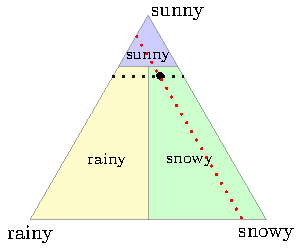
\includegraphics[width=0.3\linewidth]{tikz/t-example.pdf}
	\caption{Our meteorology example with a bias towards citizen safety.}
	\label{fig:t-example}
\end{figure}

\end{document}

%%% Local Variables:
%%% mode: latex
%%% TeX-master: t
%%% End:
